\documentclass[ xcolor = pdftex, dvipsnames, table ]{beamer}

\usetheme[compress]{Berlin}
\usecolortheme{whale}
\setlength{\parskip}{0.1in}
\usepackage{bm}
\usepackage{color}
\usepackage{graphicx}
\usepackage{xcolor}
\usepackage{tikz}
\usepackage{tabularx}
\usepackage{stackengine}
\usetikzlibrary{positioning, shapes, snakes}

%\usepackage{ctable}
%\usepackage[percent]{overpic}
%\usepackage[makeroom]{cancel}

\makeatletter
\def\hlinewd#1{
\noalign{\ifnum0=`}\fi\hrule \@height #1
\futurelet\reserve@a\@xhline}
\makeatother

%
%

\begin{document}

%
%ftp://ftp.pcouncil.org/pub/!!!Catch_Estimation_Methodology_Review_2018/

\title{\textbf{Improving Catch Estimation Methods in Sparsely Sampled, Mixed Stock Fisheries.}}

\author{
\textbf{\mbox{Nick Grunloh}}
%%$~$\\
%%\vspace{-0.5cm}
%\textbf{Nicholas Grunloh, }\\%\vspace{0.3cm}
%%\textbf{In Cooperation With:}\\
%\textbf{E.J. Dick, Don Pearson, John Field, Marc Mangel}
}

\institute[]{\textbf{UCSC :: CSTAR :: SWFSC :: NMFS}}

\date{
%$~$\\
%\vspace{-1.5cm}
%\includegraphics[width=0.45\textwidth]{./Rockfish.png}\\
\textbf{30 July 2018}
}

%
%

%
\section{Introduction}
\subsection{}
\begin{frame}
        \maketitle
\end{frame}

%
%

\begin{frame}{Diagnostic}
	Show Example
\end{frame}

%
%

%\section{}
\subsection{}
\begin{frame}{Beta-Binomial Model}
\vspace{-0.5cm}
%\begin{align*}
\begin{equation*}
        y_{ijklm\eta} \sim \text{Beta-Binomial}\Big(\mu_{jklm\eta},~\sigma^2_{jklm\eta} \Big)
\end{equation*}
\vspace{-0.7cm}
\begin{gather*}
%       \vspace{0.2cm}
        \mu_{jklm\eta} = n~\text{logit}^{-1}(\theta_{jklm\eta})\\
        %=n~\frac{\alpha_{jklm\eta}}{\alpha_{jklm\eta}+\beta_{jklm\eta}}  
        \sigma^2_{jklm\eta} = \mu_{jklm\eta}\Big(1-\frac{\mu_{jklm\eta}}{n}\Big)\Big(1+(n-1)~\rho\Big)
        %\sigma^2_{jklm\eta} = \bigg(\mu_{jklm\eta}-\frac{\mu^2_{jklm\eta}}{n}\bigg)\bigg(1+(n-1)~\rho\bigg)
%       \vspace{0.2cm}
\end{gather*}
\vspace{-0.2cm}
\begin{equation*}
        \theta_{jklm\eta} = \beta_0 + \beta^{(s)}_j + \beta^{(p)}_k + \beta^{(g)}_l + \color{blue}{\beta^{(t)}_{m\eta}}%\beta^{(y)}_m + \beta^{(q)}_\eta +
 \beta^{(y:q)}_{m\eta}   %{\color{blue}a_{jklm\eta}} + {\color{OliveGreen}b_{jklm\eta}} %+ c^*_{jklm\eta}
        %=n~\text{logit}^{-1}(\theta_{jklm\eta})
\end{equation*}
\hspace{-0.5cm}
%0.68
\begin{minipage}[h!]{0.55\textwidth}
        $~$\\
        $y_{ijklm\eta}$: $i^{\text{th}}$ sample of the $j^{\text{th}}$ species' integer weight, in the $k^{\text{th}}$ port, caught with the $l^{\text{th}}$ gear, in the $\eta^{\text{th}}$ \mbox{quarter,} of year $m$, for a particular market \mbox{category.}
\end{minipage}
\begin{minipage}{0.45\textwidth}
        \vspace{-0.5cm}
        \hspace{4cm}
        \begin{eqnarray*}
        j &\in&\left\{1, ..., J\right\} \text{Species}\\
        k &\in&\left\{1, ..., K\right\} \text{Ports}\\
        l &\in&\left\{1, ..., L\right\} \text{Gears}\\
        m &\in&\left\{1, ..., M\right\} \text{Years}\\
        \eta &\in&\left\{1, ..., H\right\} \text{Quarters}
        \end{eqnarray*}
\end{minipage}
\end{frame}

%
%

%
\section{Time Model}
\subsection{}
\begin{frame}{Time Models}
\hspace*{-0.5cm}
\begin{minipage}{0.3\textwidth}
\begin{center}
\textbf{(M1)}
\begin{eqnarray*}
&\beta^{(t)}_{m\eta} = \beta^{(y)}_{m} + \beta^{(q)}_{\eta}&\\
&\beta^{(y)}_{m} \sim N(0, 32^2)&\\
&\beta^{(q)}_{\eta} \sim N(0, 32^2)&\\
&~&
\end{eqnarray*}
\end{center}

\begin{center}
\textbf{(M4)}
\begin{eqnarray*}
&\beta^{(t)}_{m\eta} = \beta^{(y:q)}_{m\eta}&\\
&\beta^{(y:q)}_{m\eta} \sim N(0, v)&\\
&~&
\end{eqnarray*}
\end{center}
\end{minipage}
\begin{minipage}{0.3\textwidth}
\begin{center}
\textbf{(M2)}
\begin{eqnarray*}
&\beta^{(t)}_{m\eta} = \beta^{(y)}_{m} + \beta^{(q)}_{\eta}&\\
&\beta^{(y)}_{m} \sim N(0, v^{(y)})&\\
&\beta^{(q)}_{\eta} \sim N(0, v^{(q)})&\\
&~&
\end{eqnarray*}
\end{center}

\begin{center}
\textbf{(M5)}
\begin{eqnarray*}
&\beta^{(t)}_{m\eta} = \beta^{(y:q)}_{m\eta}&\\
&\beta^{(y:q)}_{m\eta} \sim N(0, v_\eta)&\\
&~&
\end{eqnarray*}
\end{center}
\end{minipage}
%\vspace*{-1cm}
\begin{minipage}{0.3\textwidth}
\begin{center}
~~~~~~~~~~~~~\textbf{(M3)}
\begin{eqnarray*}
&\beta^{(t)}_{m\eta} = \beta^{(y)}_{m} + \beta^{(q)}_{\eta} + \beta^{(y:q)}_{m\eta} & \\
&\beta^{(y)}_{m} \sim N(0, v^{(y)}) & \\
&\beta^{(q)}_{\eta} \sim N(0, v^{(q)}) & \\
&\beta^{(y:q)}_{m\eta} \sim N(0, v) &
\end{eqnarray*}
\end{center}

\begin{center}
\textbf{(M6)}
\begin{eqnarray*}
&\beta^{(t)}_{m\eta} = \beta^{(y:q)}_{m\eta}&\\
&\beta^{(y:q)}_{m\eta} \sim N(0, v_m)&\\
&&
\end{eqnarray*}
\end{center}
\end{minipage}
\end{frame}

%
%

\subsection{}
\begin{frame}{MCAT 250}
	\begin{table}[ht!]
        \centering
        \begin{tabular}[c]{@{}lcccccc@{}}
        %\toprule
        \hline
        & \href{https://github.com/gasduster99/sppComp/tree/master/sscRuns/25019781982M1}{M1} & \href{https://github.com/gasduster99/sppComp/tree/master/sscRuns/25019781982M2}{M2} & \href{https://github.com/gasduster99/sppComp/tree/master/sscRuns/25019781982M3}{M3} & \href{https://github.com/gasduster99/sppComp/tree/master/sscRuns/25019781982M4}{M4} & \href{https://github.com/gasduster99/sppComp/tree/master/sscRuns/25019781982M5}{M5} & \href{https://github.com/gasduster99/sppComp/tree/master/sscRuns/25019781982M6}{M6} \\ \hline
        \(\Delta\) DIC & 6448.98 & 0.33 & 0 & 4.45 & 9.3 & 7.42 \\
        \(\Delta\) WAIC & 6421.5 & 0.37 & 0 & 4.52 & 8.25 & 6.55 \\
        \(pr(M|y)\) & 0 & 0 & 0 & 0.03 & 0 & 0.97 \\ \hline
        \end{tabular}
        \end{table}
\end{frame}

%
%

\begin{frame}{$~~~~~~~~~~$ \href{https://github.com/gasduster99/sppComp/tree/master/sscRuns/25019781982M2}{M2} $~~~~~~~~~~~~~~~~~~~~$ \href{https://github.com/gasduster99/sppComp/tree/master/sscRuns/25019781982M3}{M3} $~~~~~~~~~~~~~~~~~~~~$ \href{https://github.com/gasduster99/sppComp/tree/master/sscRuns/25019781982M4}{M4} }	
	\begin{figure}[ht!]
        \centering
	\hspace*{-1cm}
        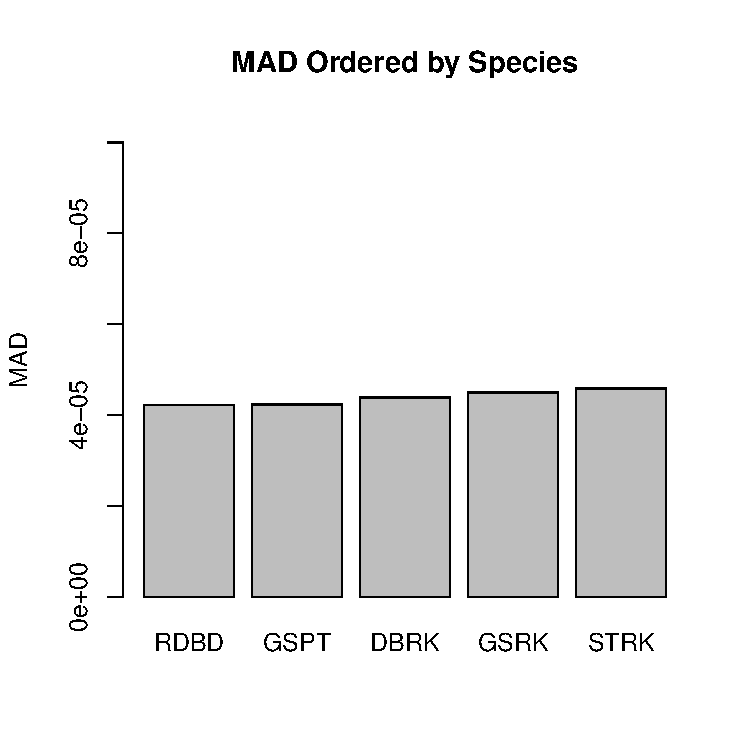
\includegraphics[width=.4\textwidth]{../sscRuns/25019781982M2/sppHeadMad68.pdf}
        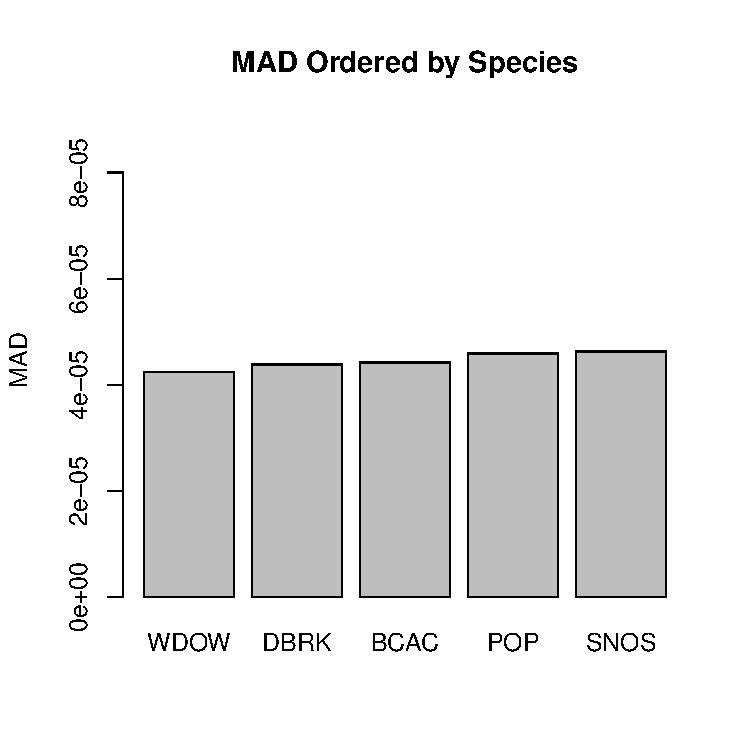
\includegraphics[width=.4\textwidth]{../sscRuns/25019781982M3/sppHeadMad68.pdf}
	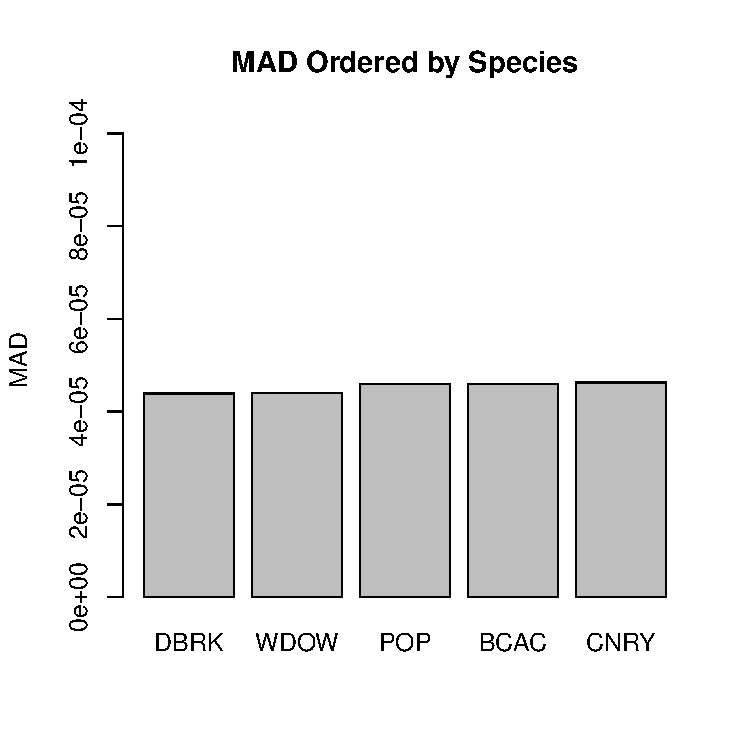
\includegraphics[width=.4\textwidth]{../sscRuns/25019781982M4/sppHeadMad68.pdf}
	\end{figure}
\end{frame}

%
%

%
\begin{frame}
        \begin{figure}[ht!]
        \centering
        \vspace{-0.75cm}
        \includegraphics[height=1.1\textheight]{{./postSSC/25019781982M2M3M4/margBCAC/margBCAC-0.68-Diagnostic}.pdf}
        \end{figure}	
\end{frame}

%
%

%
\begin{frame}
	\begin{figure}[ht!]
        \centering
	\vspace{-0.75cm}
	%\begin{minipage}[h!]{0.49\textwidth}
	%\hspace*{-1cm}
        %\includegraphics[height=1.05\textheight]{{./postSSC/25019781982M2M3M4/margBCAC/margBCAC-0.68-Diagnostic}.pdf}
	%\end{minipage}
	%\begin{minipage}[h!]{0.49\textwidth}
	\includegraphics[height=1.1\textheight]{{./postSSC/25019781982M2M3M4/margWDOW/margWDOW-0.68-Diagnostic}.pdf}
	%\end{minipage}
        \end{figure}
\end{frame}

%
%

\begin{frame}{$~~~~~~~~~~$ \href{https://github.com/gasduster99/sppComp/tree/master/sscRuns/25019781982M2}{M2} $~~~~~~~~~~~~~~~~~~~~$ \href{https://github.com/gasduster99/sppComp/tree/master/sscRuns/25019781982M3}{M3} $~~~~~~~~~~~~~~~~~~~~$ \href{https://github.com/gasduster99/sppComp/tree/master/sscRuns/25019781982M4}{M4} }	
	\begin{figure}[ht!]
        \centering
	\hspace*{-1cm}
        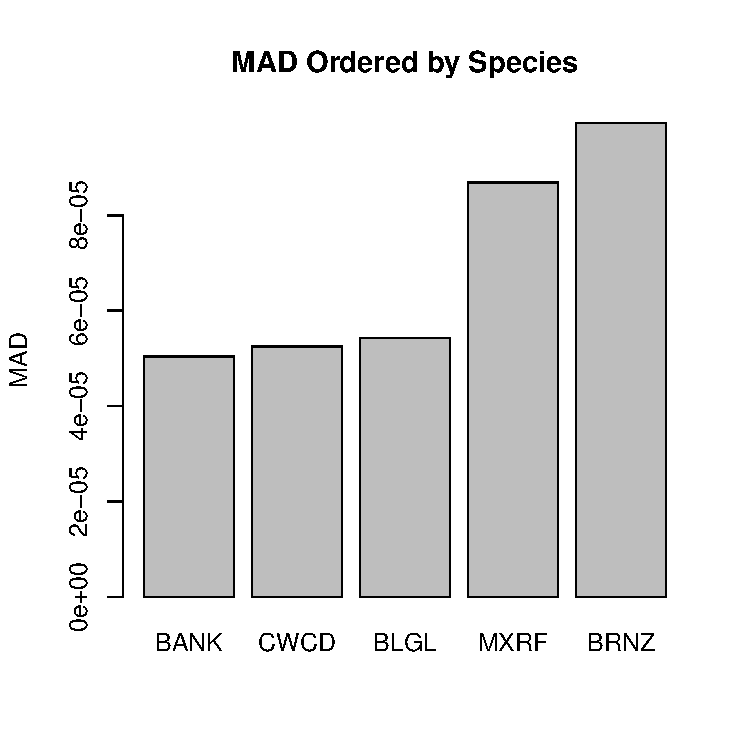
\includegraphics[width=.4\textwidth]{../sscRuns/25019781982M2/sppTailMad68.pdf}
        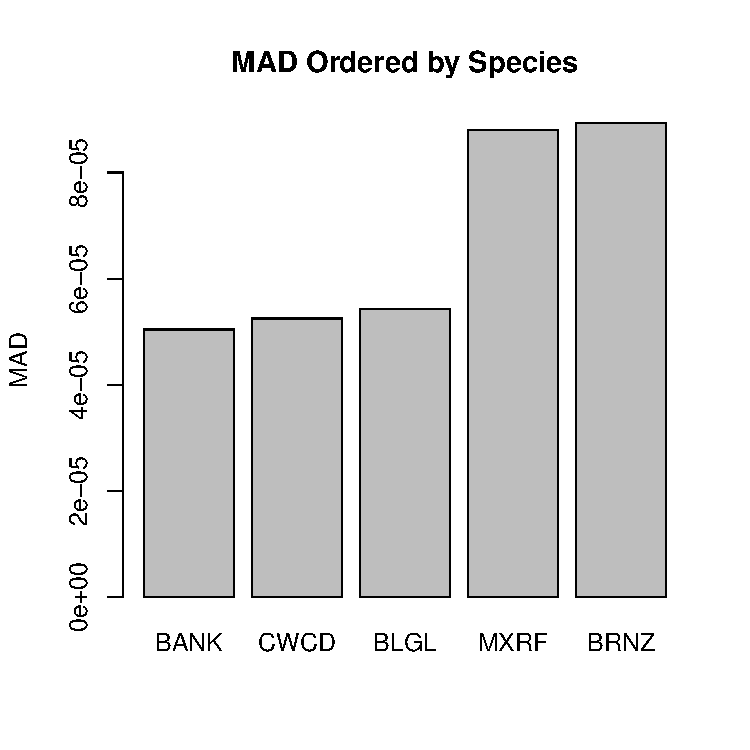
\includegraphics[width=.4\textwidth]{../sscRuns/25019781982M3/sppTailMad68.pdf}
	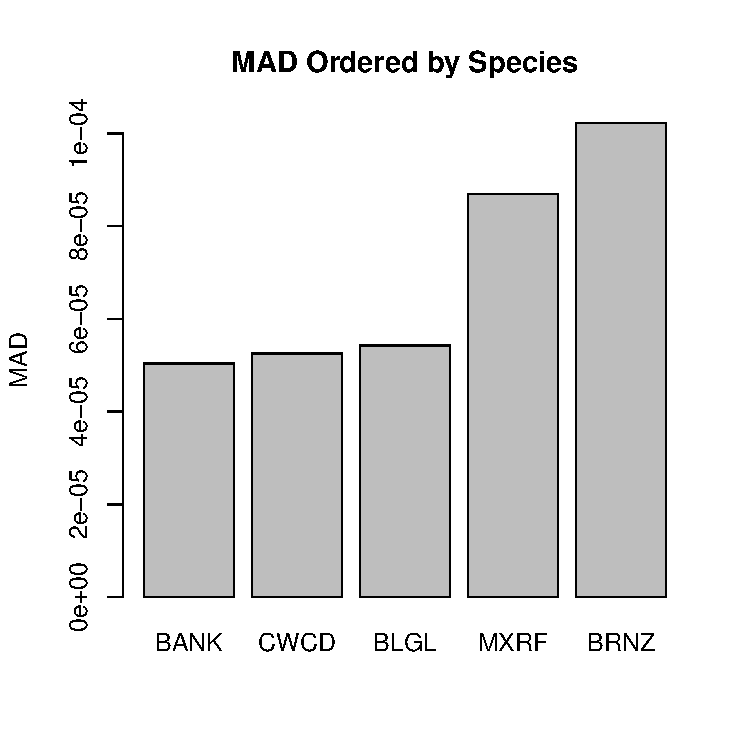
\includegraphics[width=.4\textwidth]{../sscRuns/25019781982M4/sppTailMad68.pdf}
	\end{figure}
\end{frame}

%
%

%
\begin{frame}
        \begin{figure}[ht!]
        \centering
        \vspace{-0.75cm}
        \includegraphics[height=1.1\textheight]{{./postSSC/25019781982M2M3M4/margCWCD/margCWCD-0.68-Diagnostic}.pdf}
        \end{figure}    
\end{frame}

%
%

%
\begin{frame}
        \begin{figure}[ht!]
        \centering
        \vspace{-0.75cm}
        %\begin{minipage}[h!]{0.49\textwidth}
        %\hspace*{-1cm}
        %\includegraphics[height=1.05\textheight]{{./postSSC/25019781982M2M3M4/margBCAC/margBCAC-0.68-Diagnostic}.pdf}
        %\end{minipage}
        %\begin{minipage}[h!]{0.49\textwidth}
        \includegraphics[height=1.1\textheight]{{./postSSC/25019781982M2M3M4/margMXRF/margMXRF-0.68-Diagnostic}.pdf}
        %\end{minipage}
        \end{figure}
\end{frame}

%
%

\subsection{}
\begin{frame}{MCAT 253}
	\begin{table}[ht!]
        \centering
        \begin{tabular}[c]{@{}lcccccc@{}}
        \hline
        & \href{https://github.com/gasduster99/sppComp/tree/master/sscRuns/25319781982M1}{M1} & \href{https://github.com/gasduster99/sppComp/tree/master/sscRuns/25319781982M2}{M2} & \href{https://github.com/gasduster99/sppComp/tree/master/sscRuns/25319781982M3}{M3} & \href{https://github.com/gasduster99/sppComp/tree/master/sscRuns/25319781982M4}{M4} & \href{https://github.com/gasduster99/sppComp/tree/master/sscRuns/25319781982M5}{M5} & \href{https://github.com/gasduster99/sppComp/tree/master/sscRuns/25319781982M6}{M6} \\ \hline
	\(\Delta\) DIC & 1409.81 & 0.09 & 0.1 & 0.07 & 0.05 & 0 \\                        
	\(\Delta\) WAIC & 1391.66 & 0.16 & 0.18 & 0 & 0.13 & 0.08 \\
	\(pr(M|y)\) & 0 & 0 & 0 & 1 & 0 & 0 \\ \hline
        \end{tabular}
        \end{table}
\end{frame}

%
%

\begin{frame}{$~~~~~~~~~~$ \href{https://github.com/gasduster99/sppComp/tree/master/sscRuns/25319781982M4}{M4} $~~~~~~~~~~~~~~~~~~~~$ \href{https://github.com/gasduster99/sppComp/tree/master/sscRuns/25319781982M5}{M5} $~~~~~~~~~~~~~~~~~~~~$ \href{https://github.com/gasduster99/sppComp/tree/master/sscRuns/25319781982M6}{M6} }	
	\begin{figure}[ht!]
        \centering
	\hspace*{-1cm}
        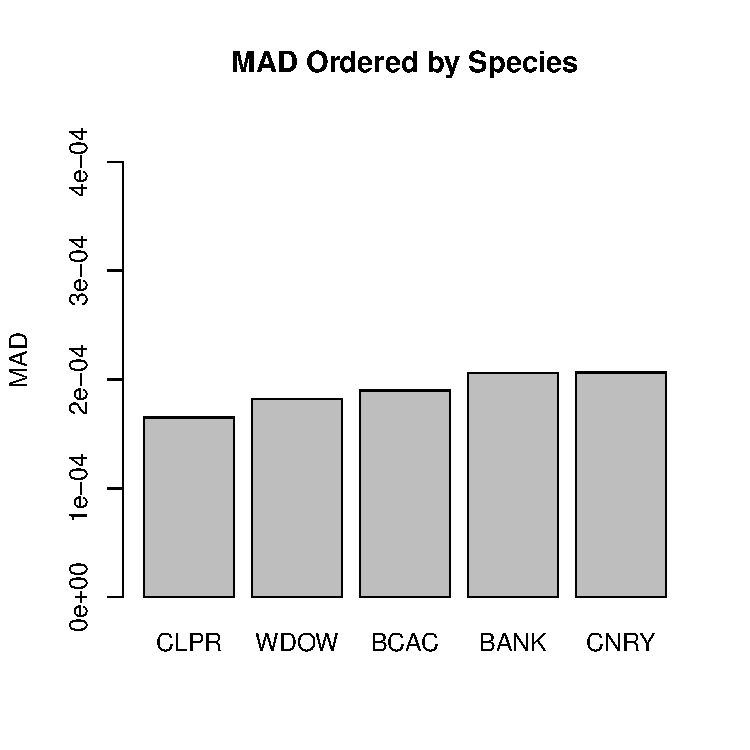
\includegraphics[width=.4\textwidth]{../sscRuns/25319781982M4/sppHeadMad68.pdf}
        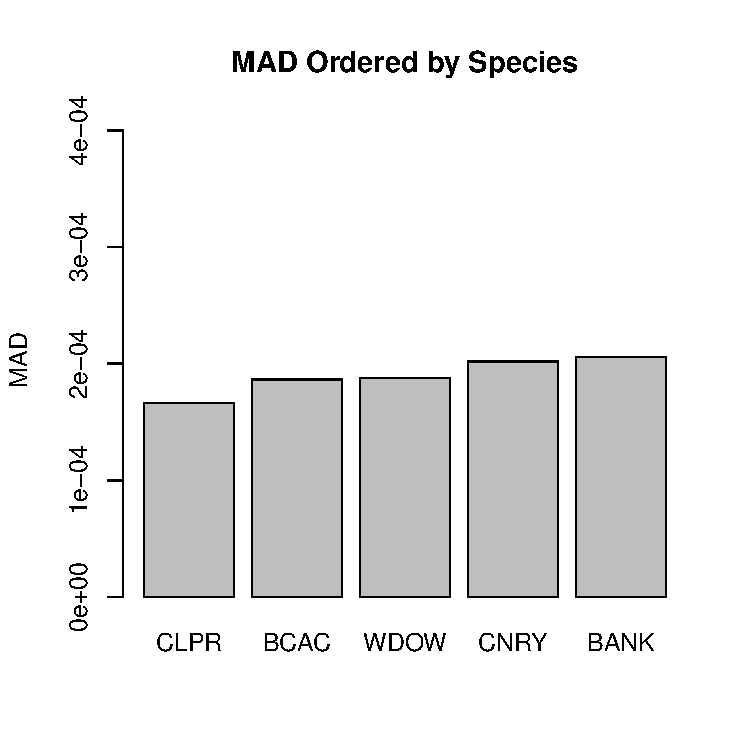
\includegraphics[width=.4\textwidth]{../sscRuns/25319781982M5/sppHeadMad68.pdf}
	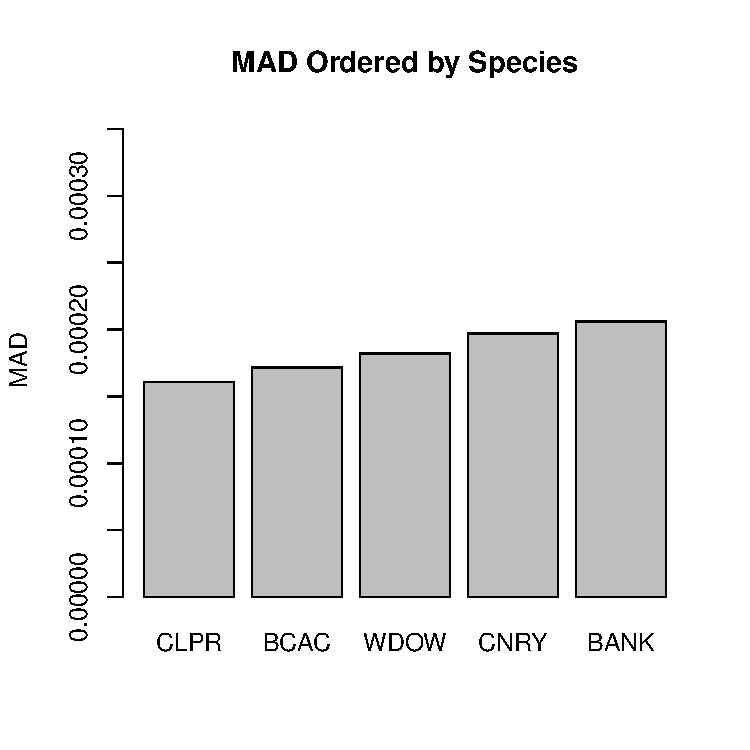
\includegraphics[width=.4\textwidth]{../sscRuns/25319781982M6/sppHeadMad68.pdf}
	\end{figure}
\end{frame}

%
%

%
\begin{frame}
        \begin{figure}[ht!]
        \centering
        \vspace{-0.75cm}
        \includegraphics[height=1.1\textheight]{{./postSSC/25319781982M4M5M6/margBCAC/margBCAC-0.68-Diagnostic}.pdf}
        \end{figure}	
\end{frame}

%
%

%
\begin{frame}
	\begin{figure}[ht!]
        \centering
	\vspace{-0.75cm}
	\includegraphics[height=1.1\textheight]{{./postSSC/25319781982M4M5M6/margWDOW/margWDOW-0.68-Diagnostic}.pdf}
	\end{figure}
\end{frame}

%
%

\begin{frame}{$~~~~~~~~~~$ \href{https://github.com/gasduster99/sppComp/tree/master/sscRuns/25319781982M4}{M4} $~~~~~~~~~~~~~~~~~~~~$ \href{https://github.com/gasduster99/sppComp/tree/master/sscRuns/25319781982M5}{M5} $~~~~~~~~~~~~~~~~~~~~$ \href{https://github.com/gasduster99/sppComp/tree/master/sscRuns/25319781982M6}{M6} }	
	\begin{figure}[ht!]
        \centering
	\hspace*{-1cm}
        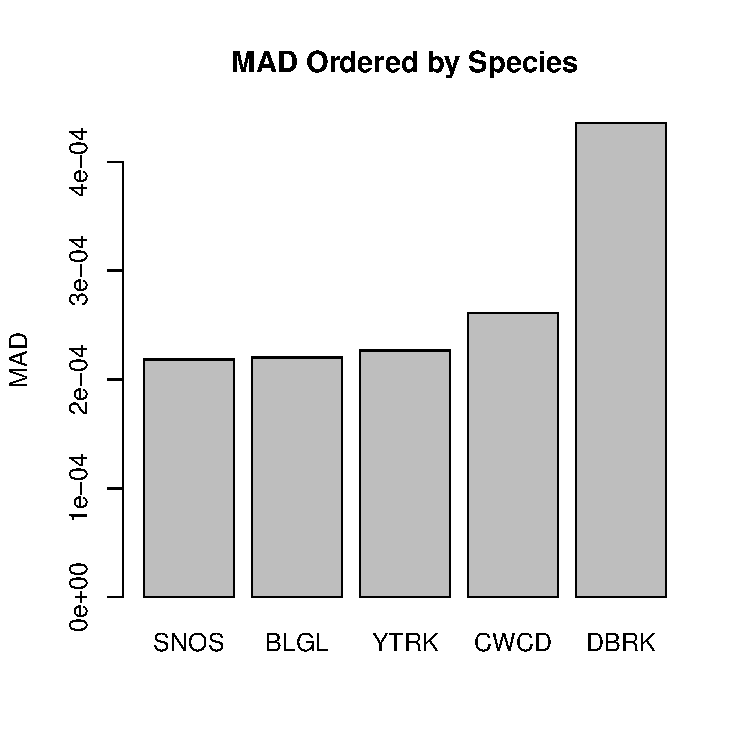
\includegraphics[width=.4\textwidth]{../sscRuns/25319781982M4/sppTailMad68.pdf}
        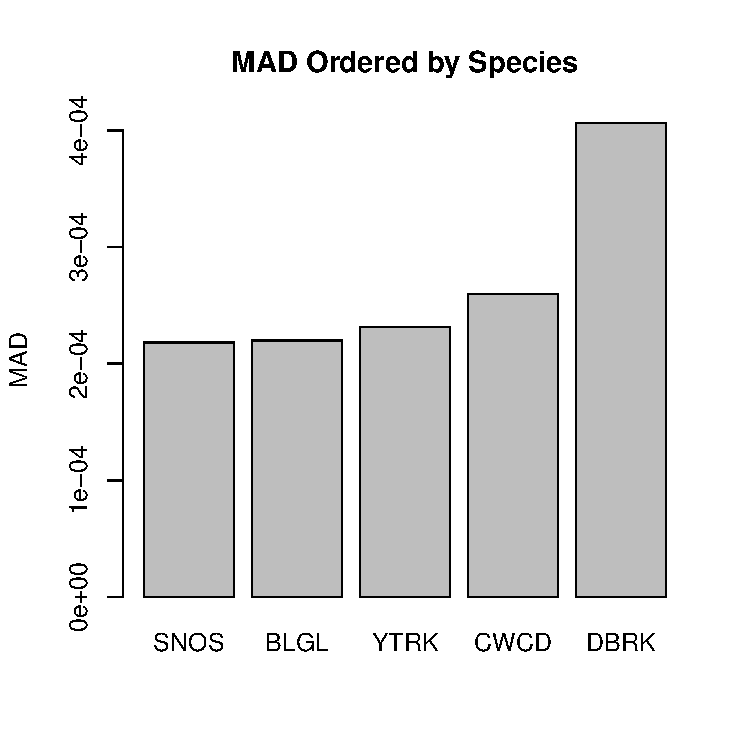
\includegraphics[width=.4\textwidth]{../sscRuns/25319781982M5/sppTailMad68.pdf}
	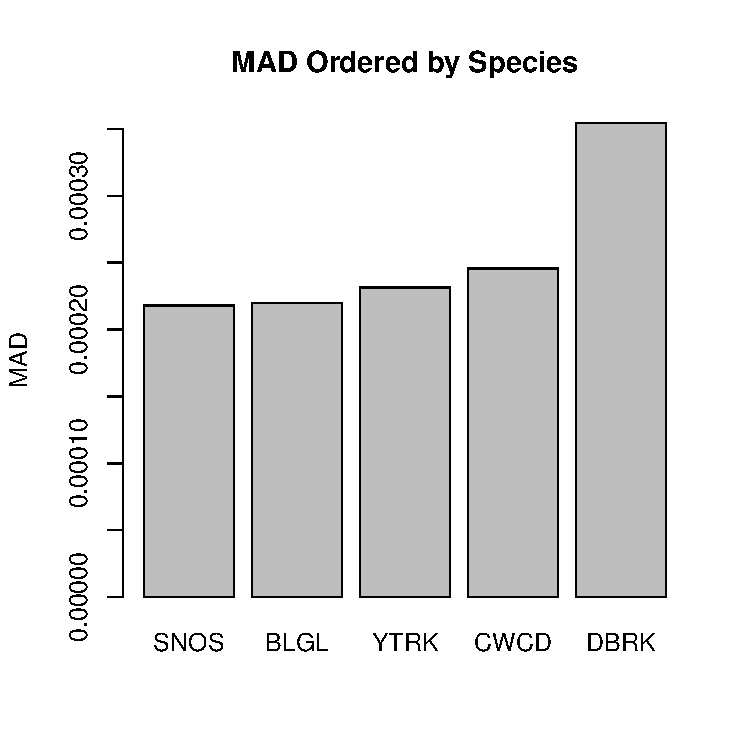
\includegraphics[width=.4\textwidth]{../sscRuns/25319781982M6/sppTailMad68.pdf}
	\end{figure}
\end{frame}

%
%

%
\begin{frame}
        \begin{figure}[ht!]
        \centering
        \vspace{-0.75cm}
        \includegraphics[height=1.1\textheight]{{./postSSC/25319781982M4M5M6/margCWCD/margCWCD-0.68-Diagnostic}.pdf}
        \end{figure}    
\end{frame}

%
%

%
\begin{frame}
        \begin{figure}[ht!]
        \centering
        \vspace{-0.75cm}
        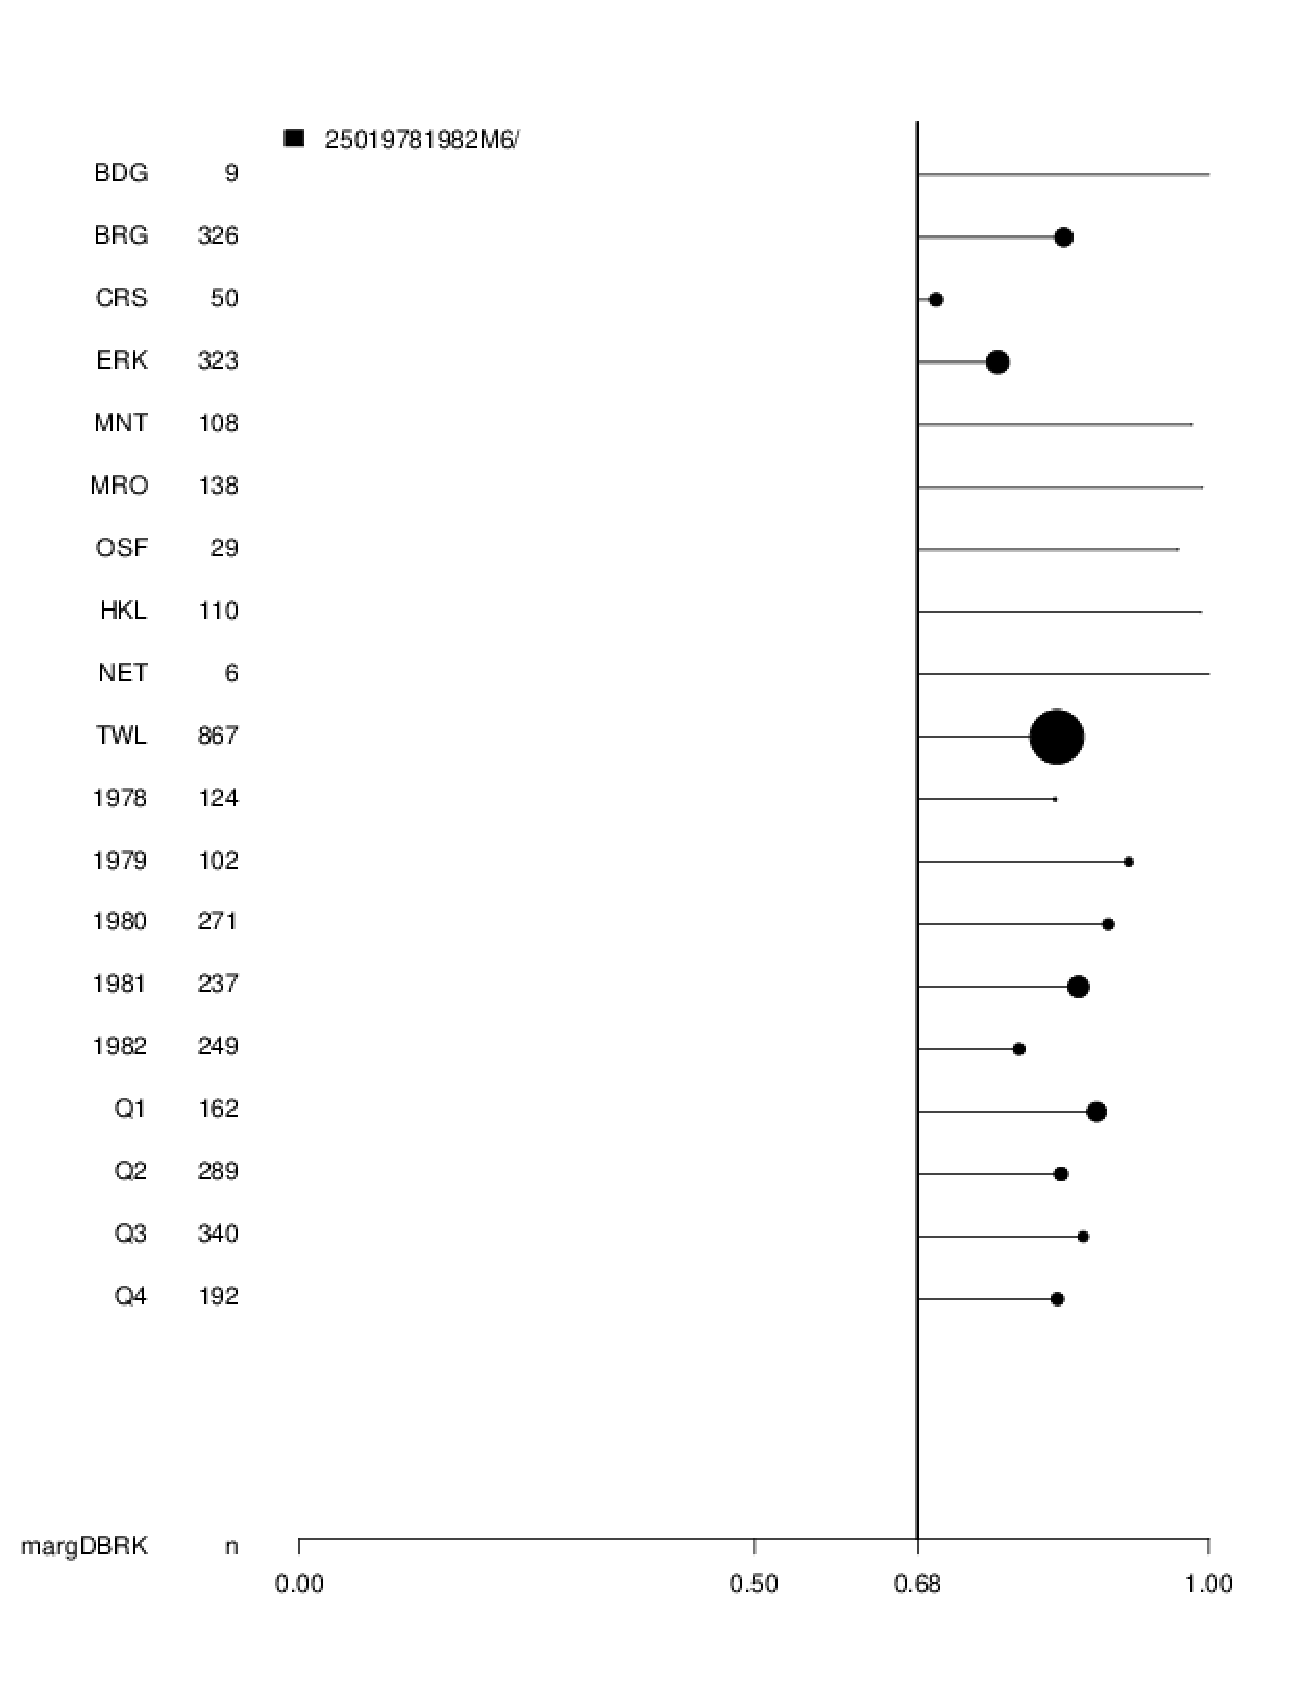
\includegraphics[height=1.1\textheight]{{./postSSC/25319781982M4M5M6/margDBRK/margDBRK-0.68-Diagnostic}.pdf}
        \end{figure}
\end{frame}

%
%

\subsection{}
\begin{frame}{MCAT 269}
	\begin{table}[ht!]
        \centering
        \begin{tabular}[c]{@{}lcccccc@{}}
        \hline
        & \href{https://github.com/gasduster99/sppComp/tree/master/sscRuns/26919781982M1}{M1} & \href{https://github.com/gasduster99/sppComp/tree/master/sscRuns/26919781982M2}{M2} & \href{https://github.com/gasduster99/sppComp/tree/master/sscRuns/26919781982M3}{M3} & \href{https://github.com/gasduster99/sppComp/tree/master/sscRuns/26919781982M4}{M4} & \href{https://github.com/gasduster99/sppComp/tree/master/sscRuns/26919781982M5}{M5} & \href{https://github.com/gasduster99/sppComp/tree/master/sscRuns/26919781982M6}{M6} \\ \hline
	\(\Delta\) DIC & 572.51 & 176.63 & 599.41 & 0.57 & 0 & 193.35 \\
	\(\Delta\) WAIC & 427.48 & 69.37 & 454.41 & 0.23 & 0 & 78.07 \\
	\(pr(M|y)\) & 0 & 0 & 0 & 0 & 0 & 1 \\ \hline
        \end{tabular}
        \end{table}
\end{frame}

%
%

\begin{frame}{$~~~~~~~~~~$ \href{https://github.com/gasduster99/sppComp/tree/master/sscRuns/26919781982M4}{M4} $~~~~~~~~~~~~~~~~~~~~$ \href{https://github.com/gasduster99/sppComp/tree/master/sscRuns/26919781982M5}{M5} $~~~~~~~~~~~~~~~~~~~~$ \href{https://github.com/gasduster99/sppComp/tree/master/sscRuns/26919781982M6}{M6} }	
	\begin{figure}[ht!]
        \centering
	\hspace*{-1cm}
        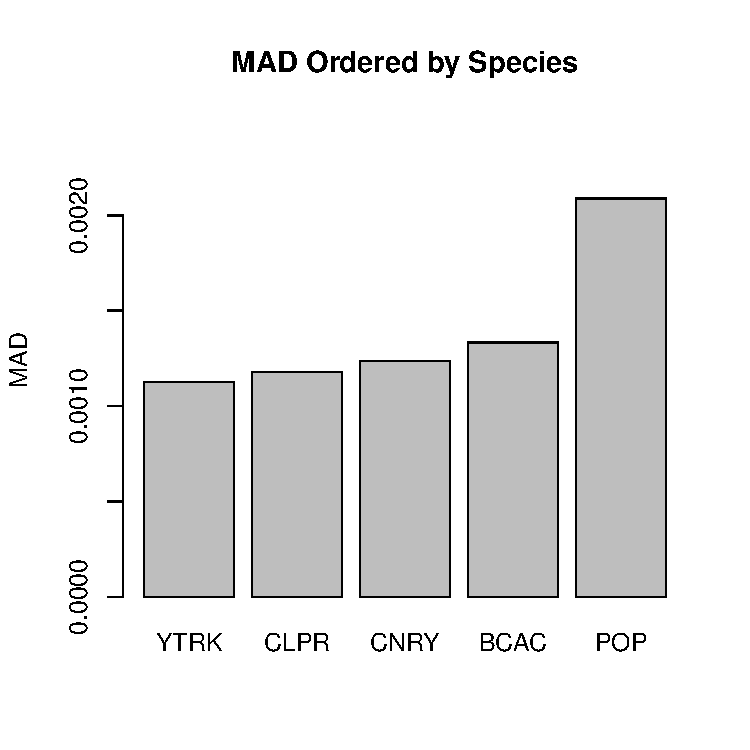
\includegraphics[width=.4\textwidth]{../sscRuns/26919781982M4/sppHeadMad68.pdf}
        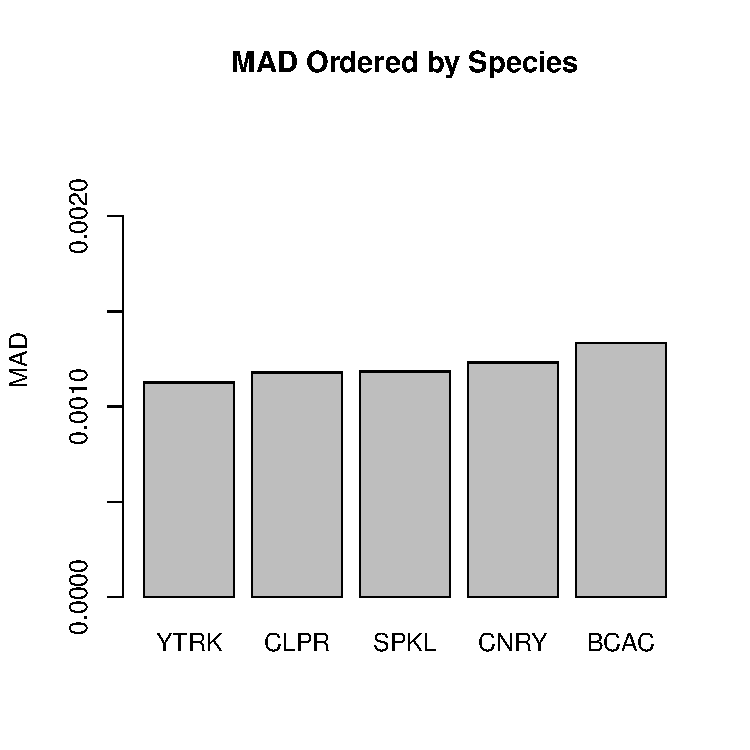
\includegraphics[width=.4\textwidth]{../sscRuns/26919781982M5/sppHeadMad68.pdf}
	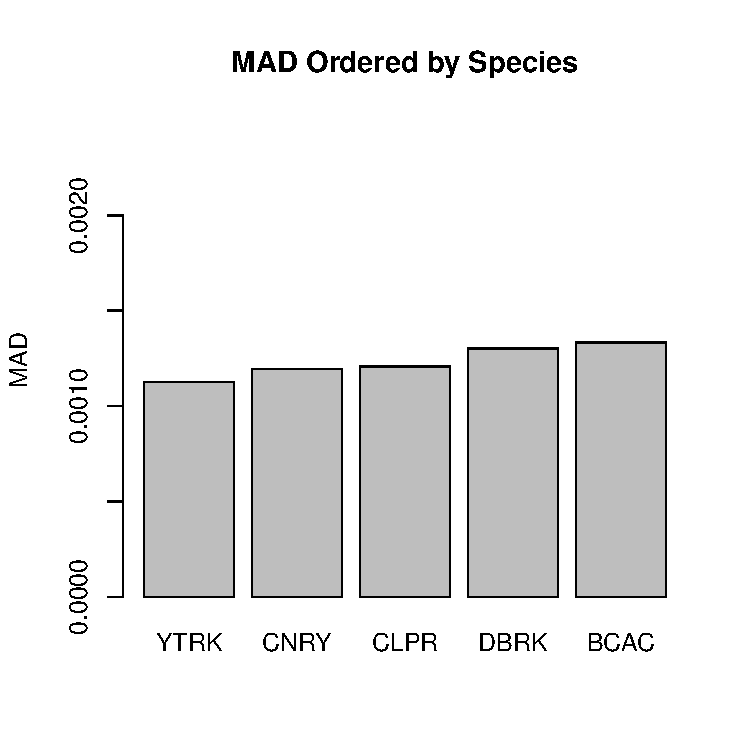
\includegraphics[width=.4\textwidth]{../sscRuns/26919781982M6/sppHeadMad68.pdf}
	\end{figure}
\end{frame}

%
%

%
\begin{frame}
        \begin{figure}[ht!]
        \centering
        \vspace{-0.75cm}
        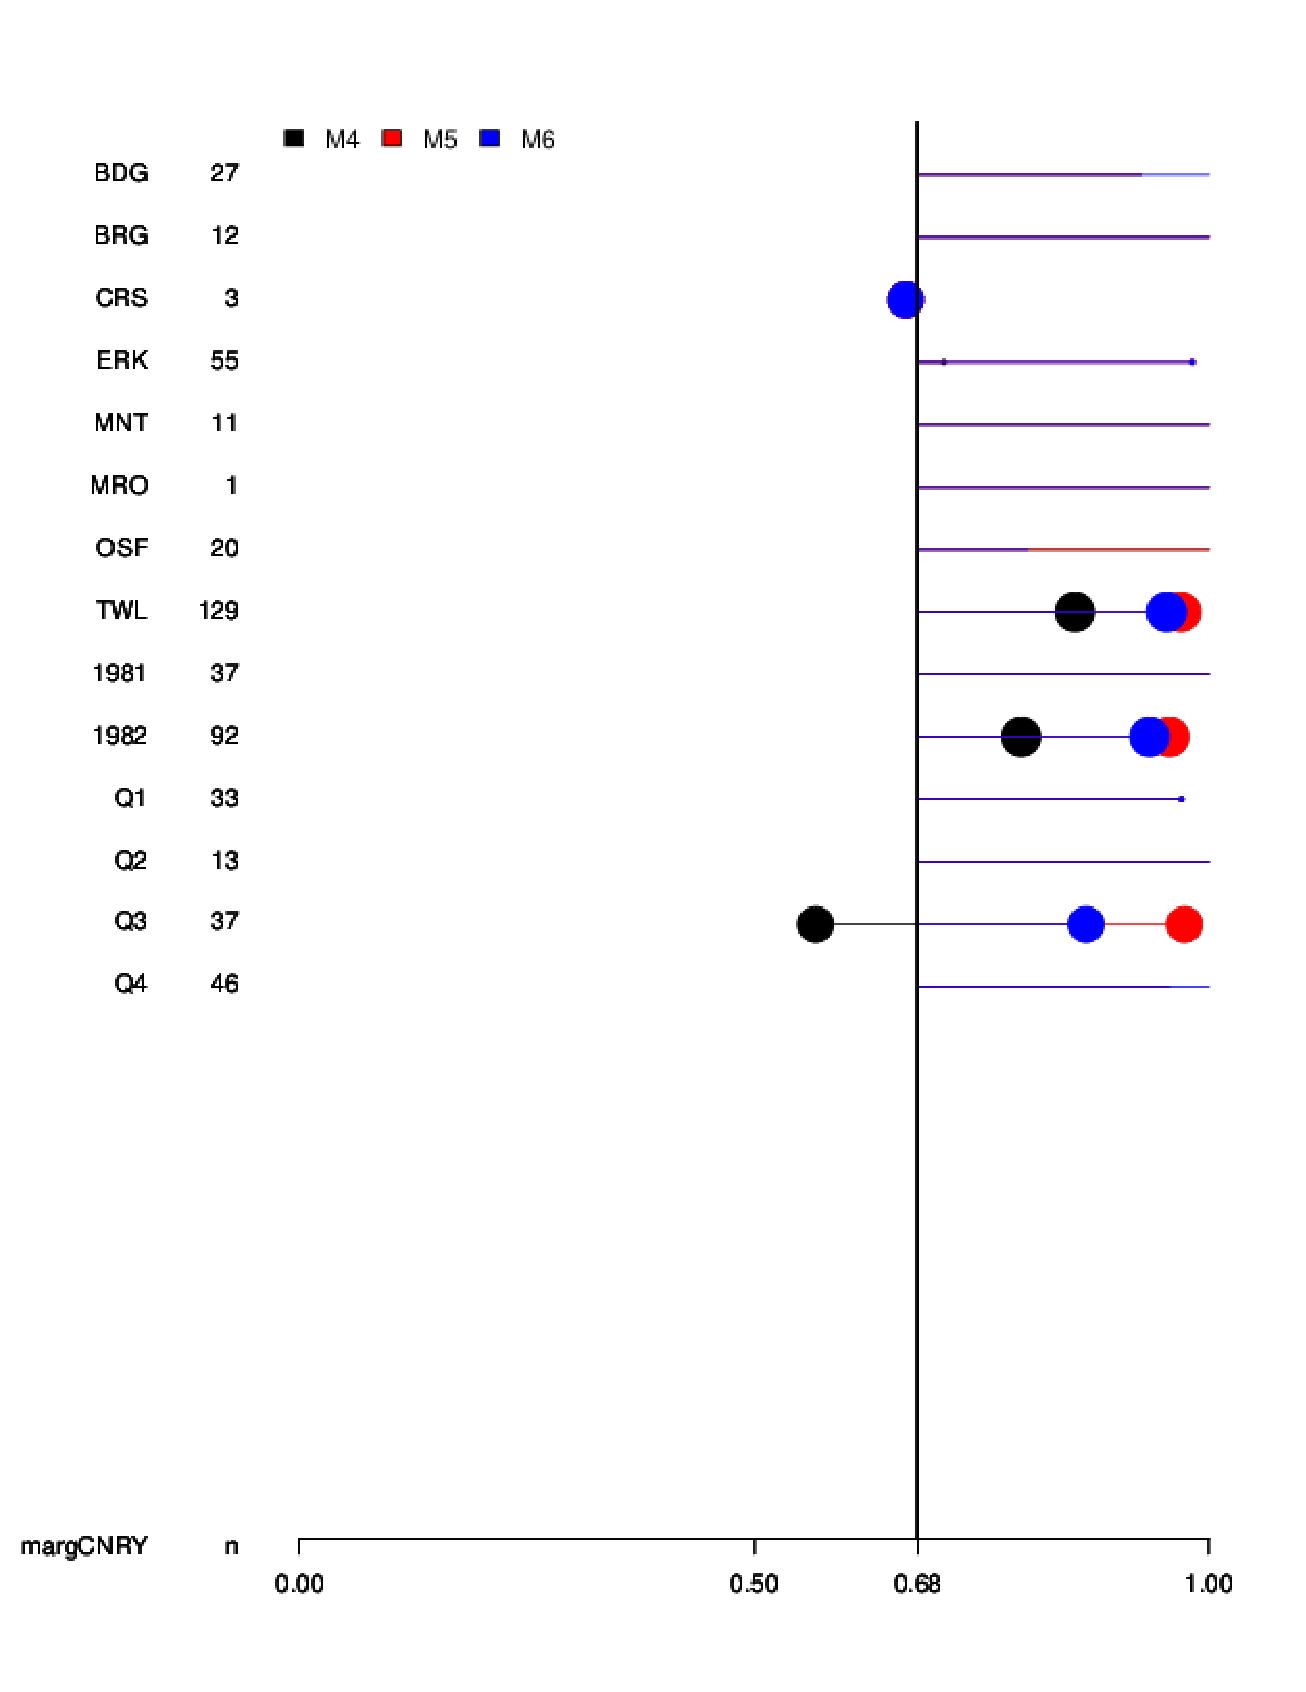
\includegraphics[height=1.1\textheight]{{./postSSC/26919781982M4M5M6/margCNRY/margCNRY-0.68-Diagnostic}.pdf}
        \end{figure}	
\end{frame}

%
%

%
\begin{frame}
        \begin{figure}[ht!]
        \centering
        \vspace{-0.75cm}
        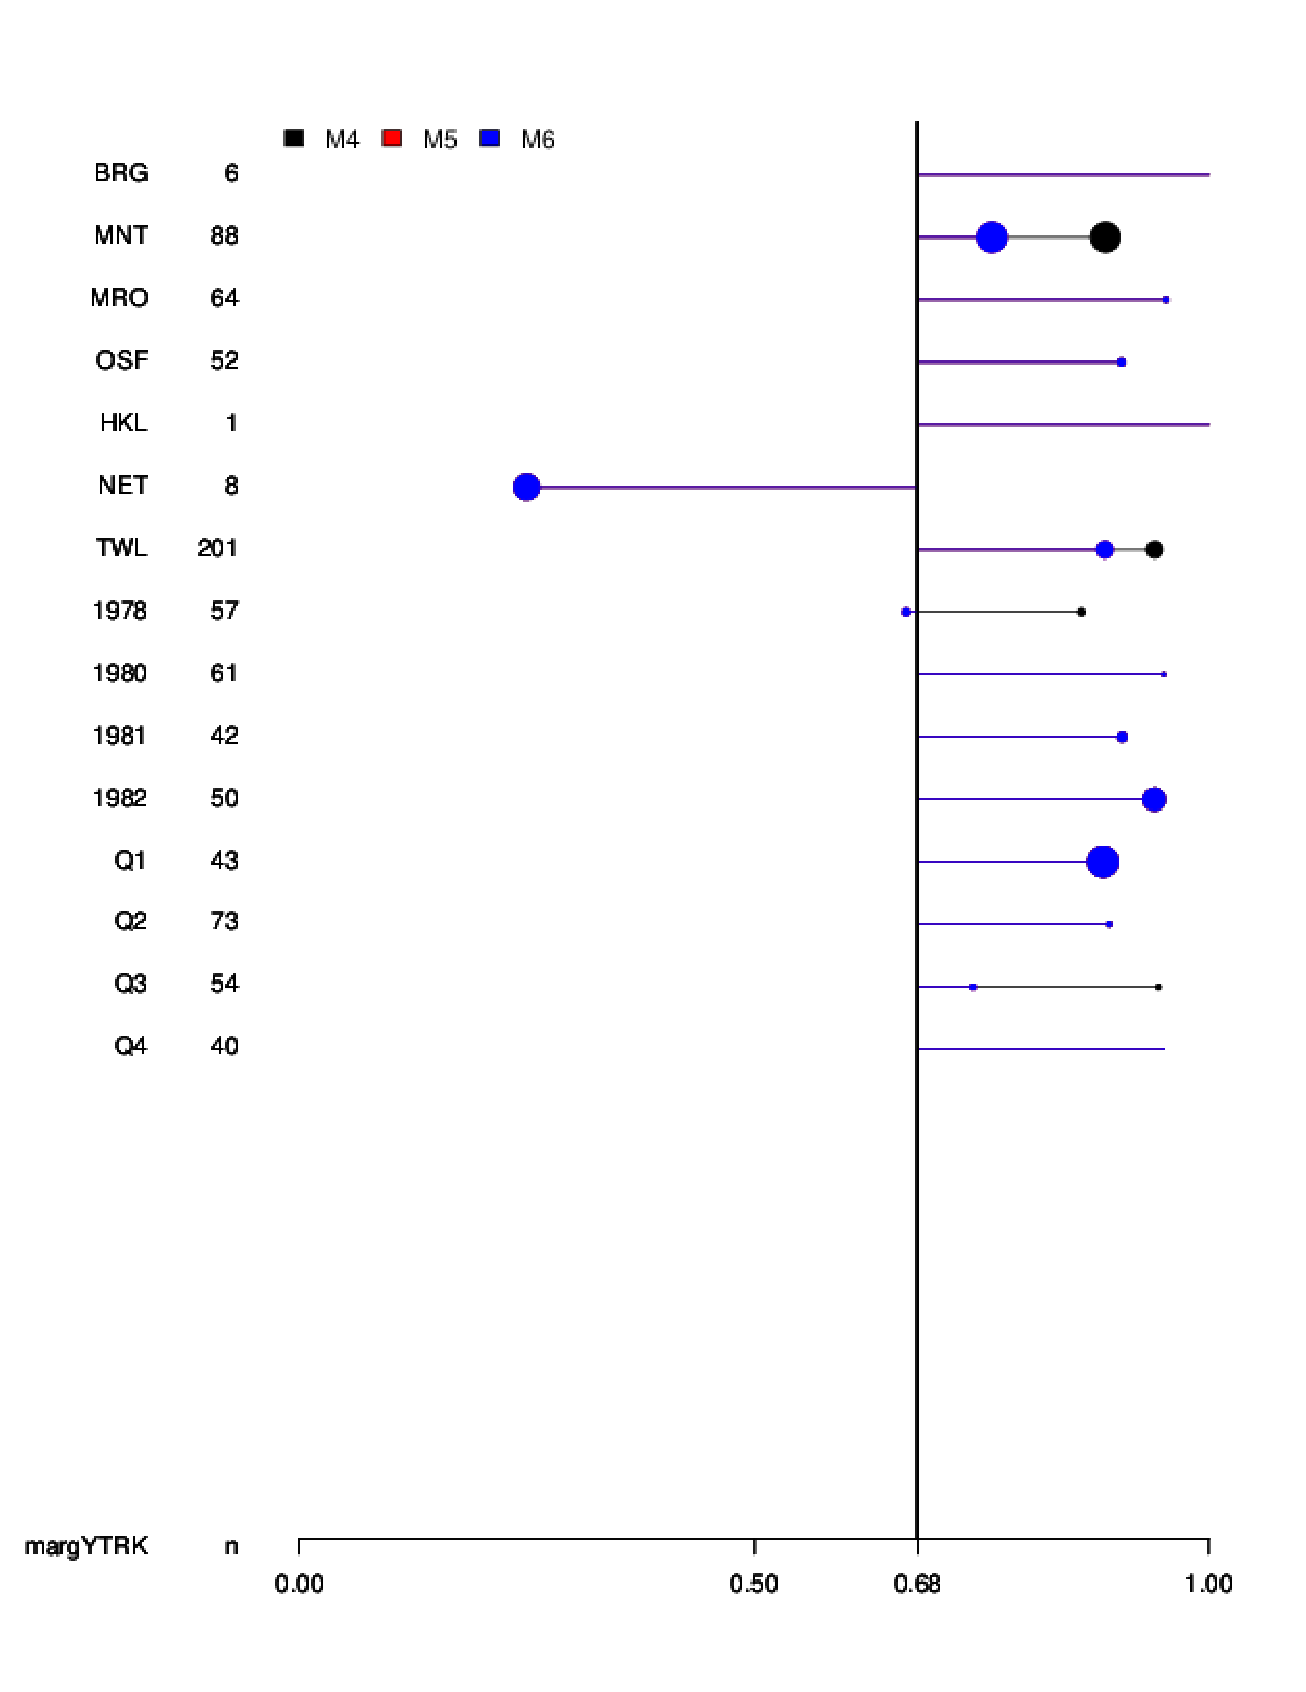
\includegraphics[height=1.1\textheight]{{./postSSC/26919781982M4M5M6/margYTRK/margYTRK-0.68-Diagnostic}.pdf}
        \end{figure}	
\end{frame}

%
%

\begin{frame}{$~~~~~~~~~~$ \href{https://github.com/gasduster99/sppComp/tree/master/sscRuns/26919781982M4}{M4} $~~~~~~~~~~~~~~~~~~~~$ \href{https://github.com/gasduster99/sppComp/tree/master/sscRuns/26919781982M5}{M5} $~~~~~~~~~~~~~~~~~~~~$ \href{https://github.com/gasduster99/sppComp/tree/master/sscRuns/26919781982M6}{M6} }	
	\begin{figure}[ht!]
        \centering
	\hspace*{-1cm}
        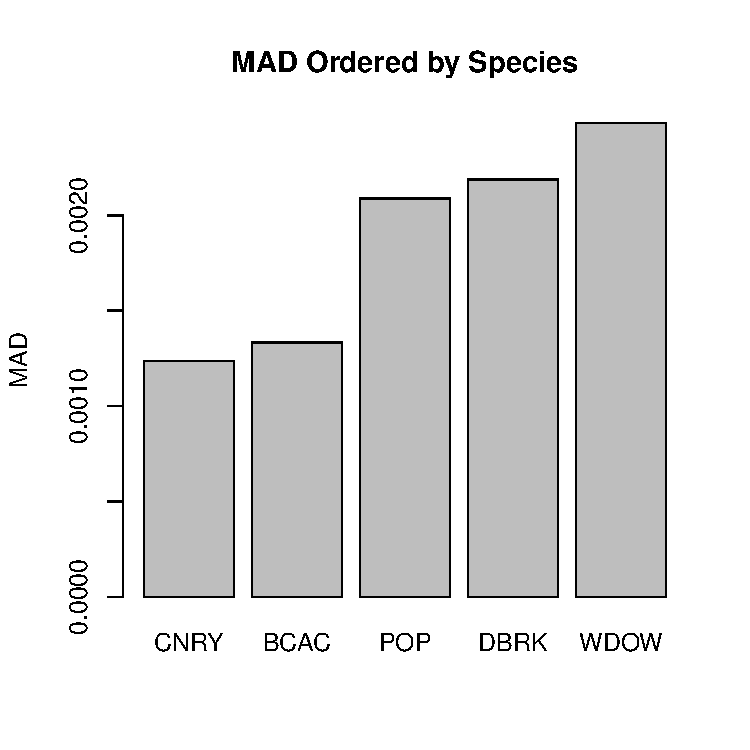
\includegraphics[width=.4\textwidth]{../sscRuns/26919781982M4/sppTailMad68.pdf}
        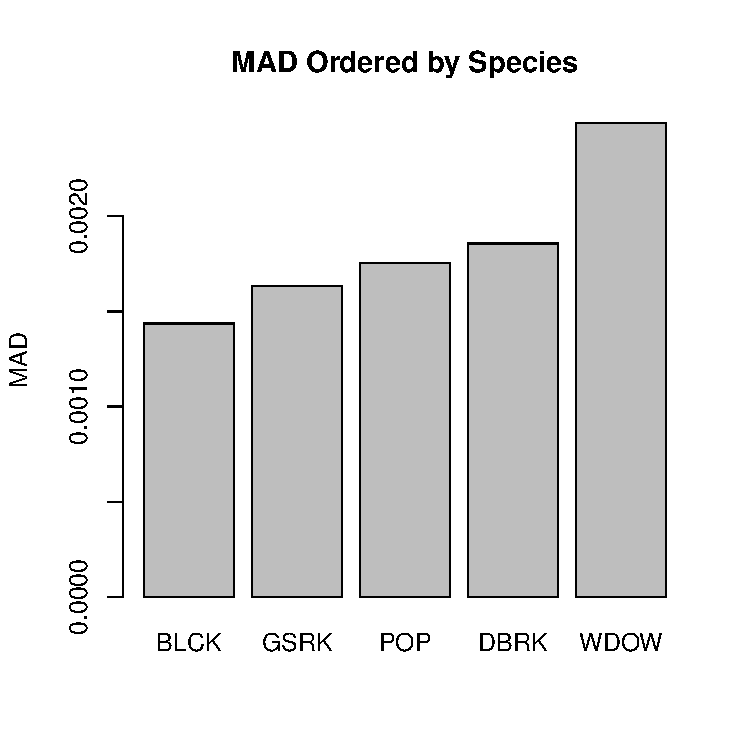
\includegraphics[width=.4\textwidth]{../sscRuns/26919781982M5/sppTailMad68.pdf}
	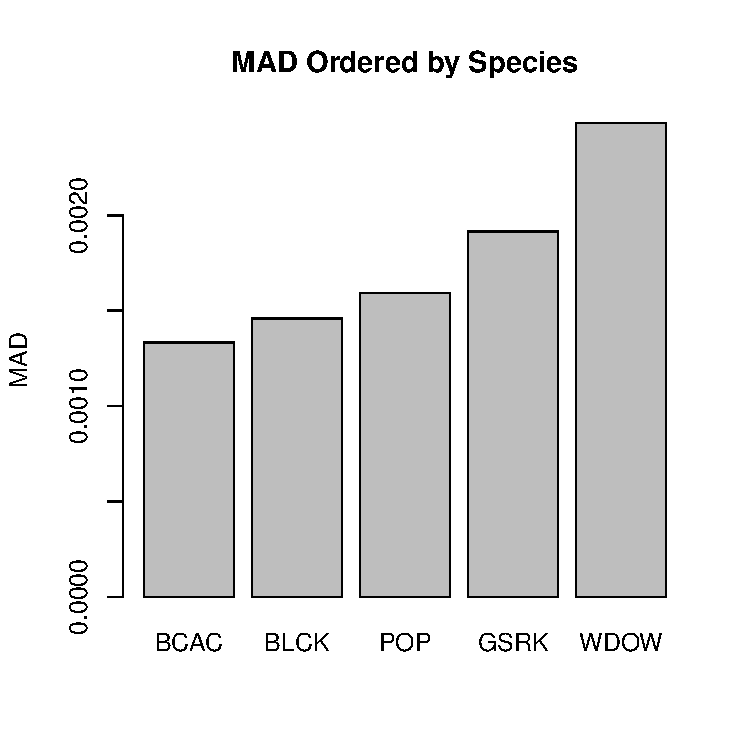
\includegraphics[width=.4\textwidth]{../sscRuns/26919781982M6/sppTailMad68.pdf}
	\end{figure}
\end{frame}

%
%

%
\begin{frame}
        \begin{figure}[ht!]
        \centering
        \vspace{-0.75cm}
        \includegraphics[height=1.1\textheight]{{./postSSC/26919781982M4M5M6/margBCAC/margBCAC-0.68-Diagnostic}.pdf}
        \end{figure}    
\end{frame}

%
%

%
\begin{frame}
        \begin{figure}[ht!]
        \centering
        \vspace{-0.75cm}
        \includegraphics[height=1.1\textheight]{{./postSSC/26919781982M4M5M6/margWDOW/margWDOW-0.68-Diagnostic}.pdf}
        \end{figure}
\end{frame}

%
%

\section{Prior Model}
\subsection{}
\begin{frame}{Priors}
$~$
\hspace*{-1.5cm}
\begin{minipage}{0.55\textwidth}
%\vspace{-0.5cm}
\begin{align*}
\beta_0 &\propto 1\\
\beta^{(s)}_j &\sim N(0, 32^2)\\
\beta^{(p)}_k &\sim N(0, 32^2)\\
\beta^{(g)}_l &\sim N(0, 32^2)\\
&\\
\text{logit}(\rho) &\sim N(0, 2^2)\\
&\\
v\sim IG(1,~&2x10^{3}) ~~~\forall~~~v 
\end{align*}
\end{minipage}
\begin{minipage}{0.4\textwidth}
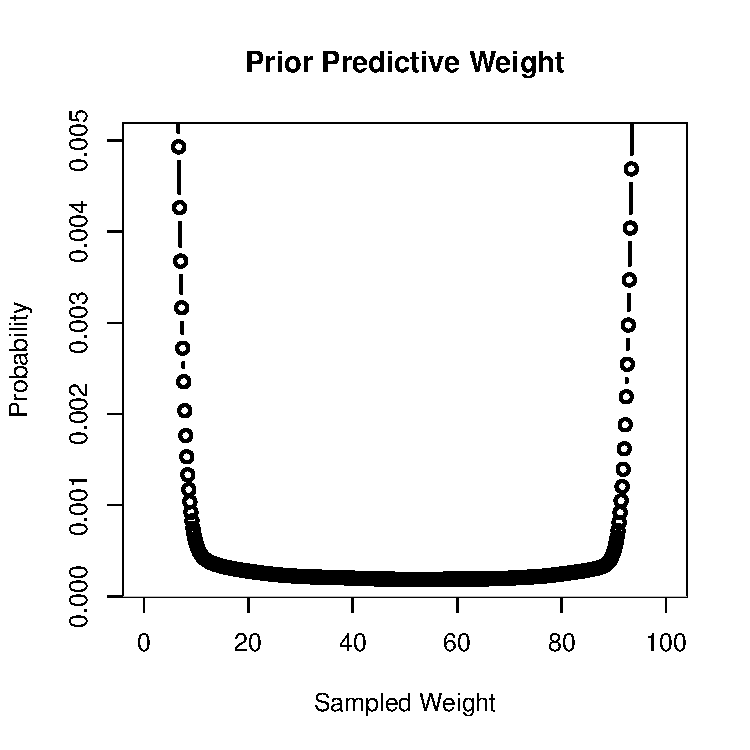
\includegraphics[width=1.4\textwidth]{pictures/priorPredict.pdf}
\end{minipage}
\end{frame}

%
%

\subsection{}
\begin{frame}{MCAT 250}
        \begin{table}[ht!]
        \centering
        \begin{tabular}[c]{@{}lcccccc@{}}
        %\toprule
        \hline
        & \href{https://github.com/gasduster99/sppComp/tree/master/sscRuns/25019781982M4}{M4} & \href{https://github.com/gasduster99/sppComp/tree/master/sscRuns/25019781982M4HC1}{M4HC1} & \href{https://github.com/gasduster99/sppComp/tree/master/sscRuns/25019781982M4HC3}{M4HC3} & \href{https://github.com/gasduster99/sppComp/tree/master/sscRuns/25019781982M4U4}{M4U4} \\ \hline
        \(\Delta\) DIC & 3.87 & 0.02 & 0.1 & 0 \\                                         
	\(\Delta\) WAIC & 3.78 & 0.03 & 0.11 & 0 \\                                       
	\(pr(M|y)\) & 0 & 0.21 & 0.37 & 0.42 \\ \hline
	\end{tabular}
        \end{table}
\end{frame}

%
%

\begin{frame}{$~~~~~~~$ \href{https://github.com/gasduster99/sppComp/tree/master/sscRuns/25019781982M4HC1}{M4HC1} $~~~~~~~~~~~~~~$ \href{https://github.com/gasduster99/sppComp/tree/master/sscRuns/25019781982M4HC3}{M4HC3} $~~~~~~~~~~~~~~~~~$ \href{https://github.com/gasduster99/sppComp/tree/master/sscRuns/25019781982M4U4}{M4U4} }
        \begin{figure}[ht!]
        \centering
        \hspace*{-1cm}
        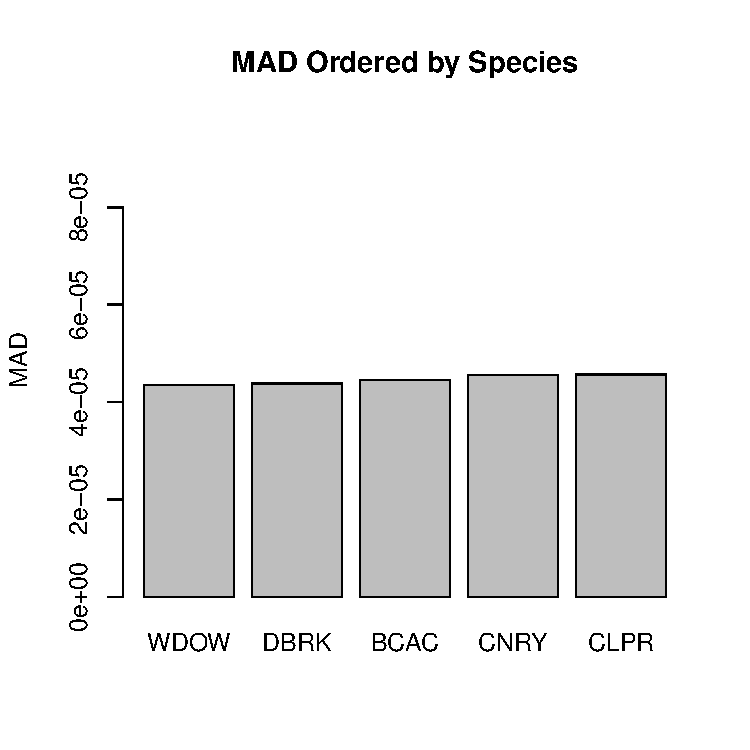
\includegraphics[width=.4\textwidth]{../sscRuns/25019781982M4HC1/sppHeadMad68.pdf}
        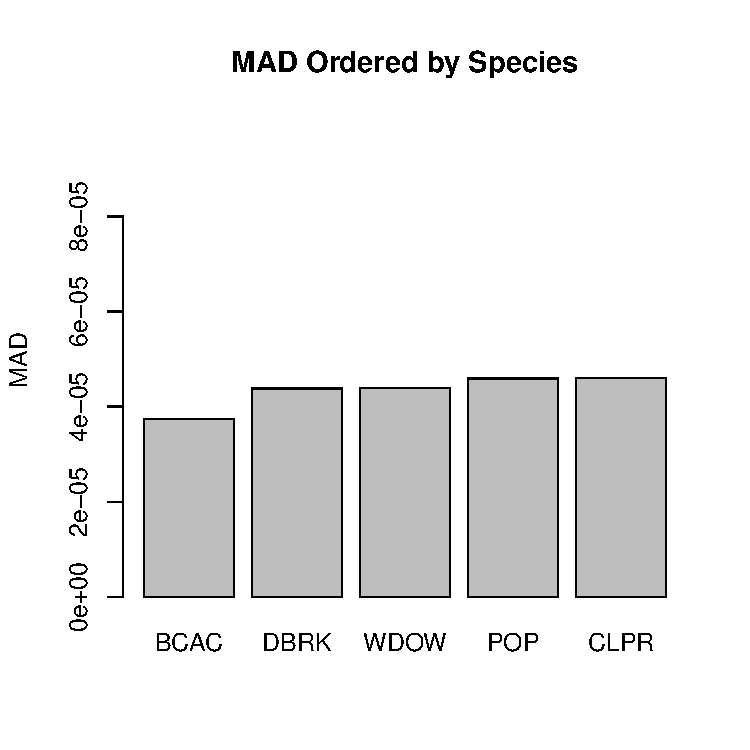
\includegraphics[width=.4\textwidth]{../sscRuns/25019781982M4HC3/sppHeadMad68.pdf}
        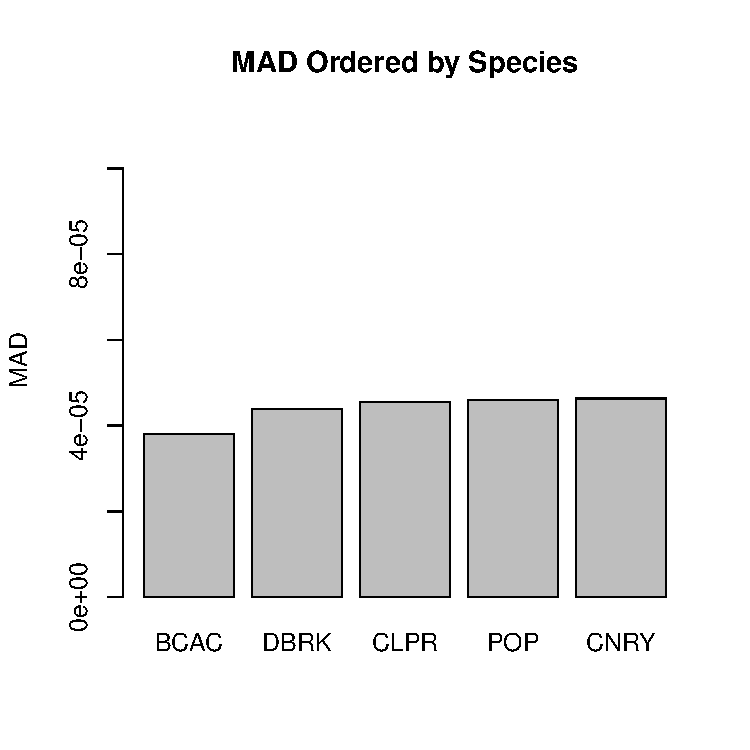
\includegraphics[width=.4\textwidth]{../sscRuns/25019781982M4U4/sppHeadMad68.pdf}
        \end{figure}
\end{frame}

%
%

%
\begin{frame}
        \begin{figure}[ht!]
        \centering
        \vspace{-0.75cm}
        \includegraphics[height=1.1\textheight]{{./postSSC/25019781982M4HC1HC3U4/margBCAC/margBCAC-0.68-Diagnostic}.pdf}
        \end{figure}   
\end{frame}

%
%

%
\begin{frame}
       \begin{figure}[ht!]
       \centering
       \vspace{-0.75cm}
       \includegraphics[height=1.1\textheight]{{./postSSC/25019781982M4HC1HC3U4/margWDOW/margWDOW-0.68-Diagnostic}.pdf}
       \end{figure}
\end{frame}

%
%

\begin{frame}{$~~~~~~~$ \href{https://github.com/gasduster99/sppComp/tree/master/sscRuns/25019781982M4HC1}{M4HC1} $~~~~~~~~~~~~~~$ \href{https://github.com/gasduster99/sppComp/tree/master/sscRuns/25019781982M4HC3}{M4HC3} $~~~~~~~~~~~~~~~~~$ \href{https://github.com/gasduster99/sppComp/tree/master/sscRuns/25019781982M4U4}{M4U4} }
        \begin{figure}[ht!]
        \centering
        \hspace*{-1cm}
        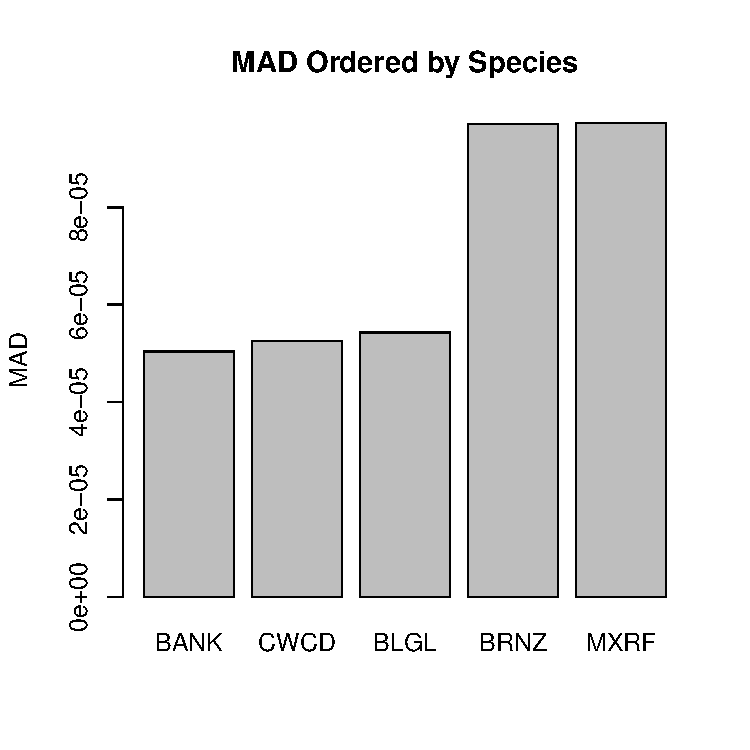
\includegraphics[width=.4\textwidth]{../sscRuns/25019781982M4HC1/sppTailMad68.pdf}
        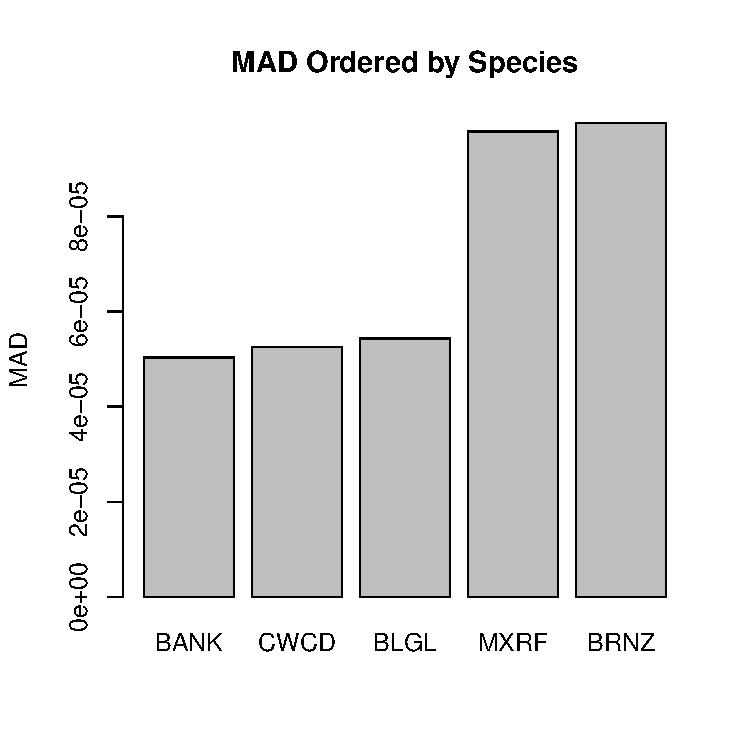
\includegraphics[width=.4\textwidth]{../sscRuns/25019781982M4HC3/sppTailMad68.pdf}
        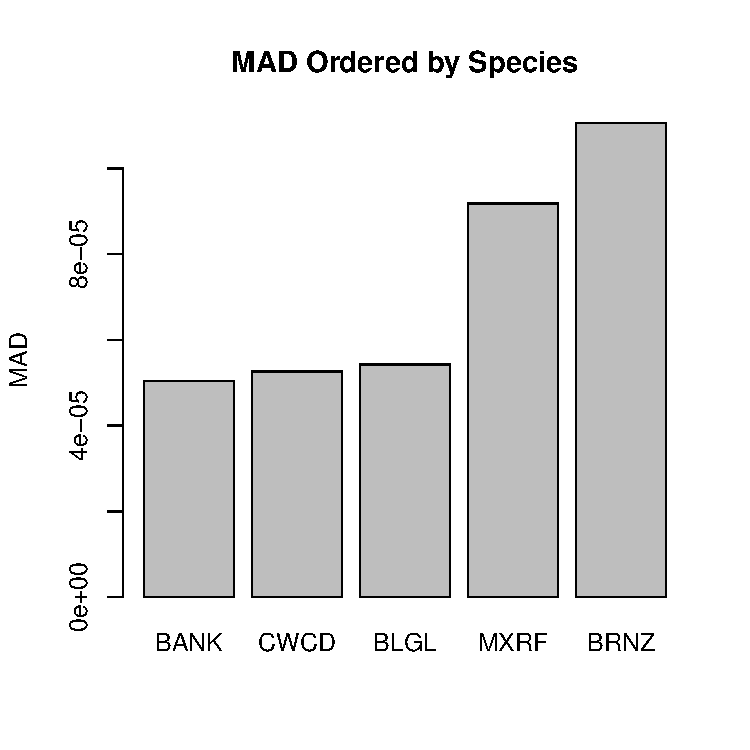
\includegraphics[width=.4\textwidth]{../sscRuns/25019781982M4U4/sppTailMad68.pdf}
        \end{figure}
\end{frame}

%
%

%
\begin{frame}
        \begin{figure}[ht!]
        \centering
        \vspace{-0.75cm}
        \includegraphics[height=1.1\textheight]{{./postSSC/25019781982M4HC1HC3U4/margCWCD/margCWCD-0.68-Diagnostic}.pdf}
        \end{figure}   
\end{frame}

%
%

%
\begin{frame}
       \begin{figure}[ht!]
       \centering
       \vspace{-0.75cm}
       \includegraphics[height=1.1\textheight]{{./postSSC/25019781982M4HC1HC3U4/margMXRF/margMXRF-0.68-Diagnostic}.pdf}
       \end{figure}
\end{frame}

%
%

\subsection{}
\begin{frame}{MCAT 253}
        \begin{table}[ht!]
        \centering
        \begin{tabular}[c]{@{}lcccccc@{}}
        %\toprule
        \hline
        & \href{https://github.com/gasduster99/sppComp/tree/master/sscRuns/25319781982M4}{M4} & \href{https://github.com/gasduster99/sppComp/tree/master/sscRuns/25319781982M4HC1}{M4HC1} & \href{https://github.com/gasduster99/sppComp/tree/master/sscRuns/25319781982M4HC3}{M4HC3} & \href{https://github.com/gasduster99/sppComp/tree/master/sscRuns/25319781982M4U4}{M4U4} \\ \hline
	\(\Delta\) DIC & 0.88 & 0.8 & 0.8 & 0 \\                                          
	\(\Delta\) WAIC & 0.76 & 0.83 & 0.83 & 0 \\                                       
	\(pr(M|y)\) & 0.01 & 0.99 & 0 & 0 \\ \hline 
	\end{tabular}
        \end{table}
\end{frame}

%
%

\begin{frame}{$~~~~~~~$ \href{https://github.com/gasduster99/sppComp/tree/master/sscRuns/25319781982M4HC1}{M4HC1} $~~~~~~~~~~~~~~$ \href{https://github.com/gasduster99/sppComp/tree/master/sscRuns/25319781982M4HC3}{M4HC3} $~~~~~~~~~~~~~~~~~$ \href{https://github.com/gasduster99/sppComp/tree/master/sscRuns/25319781982M4U4}{M4U4} }
        \begin{figure}[ht!]
        \centering
        \hspace*{-1cm}
        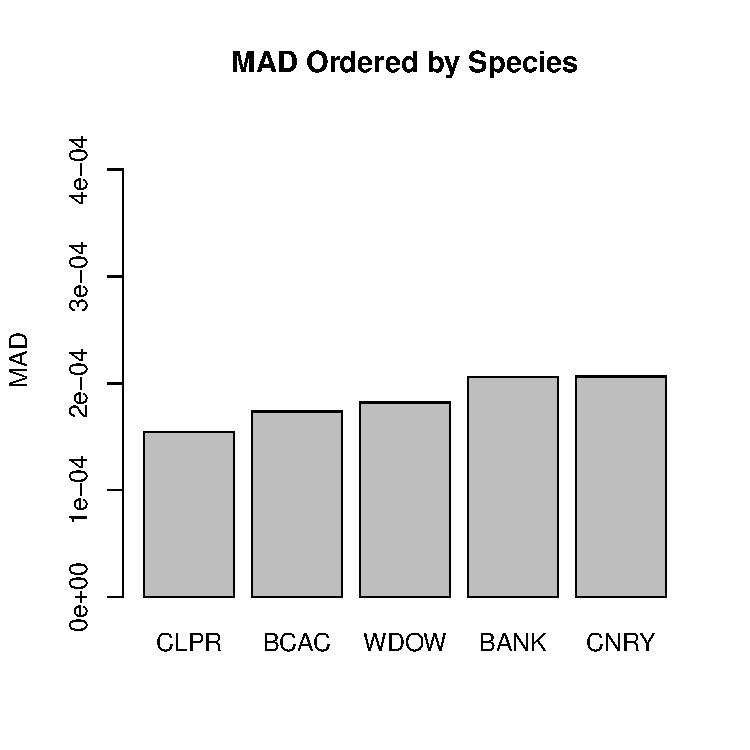
\includegraphics[width=.4\textwidth]{../sscRuns/25319781982M4HC1/sppHeadMad68.pdf}
        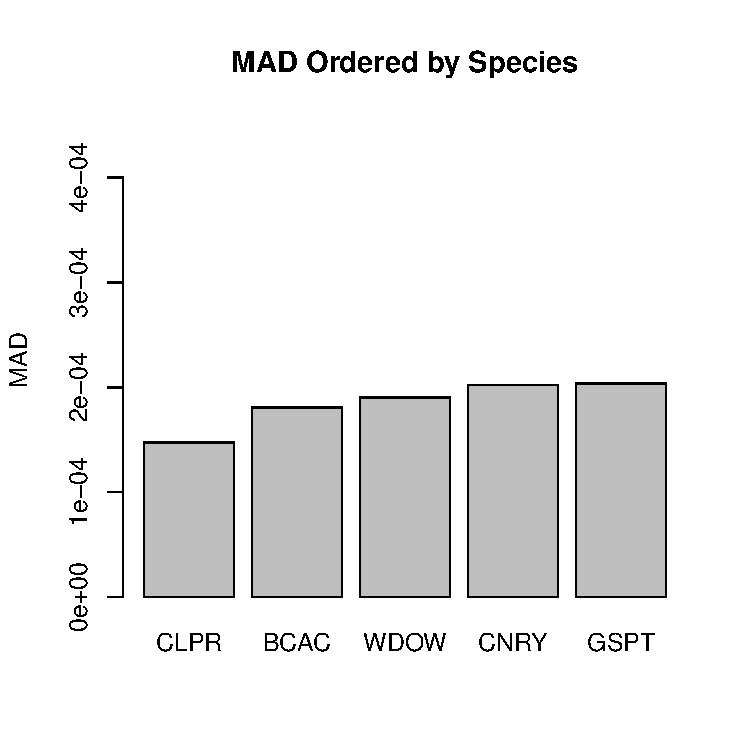
\includegraphics[width=.4\textwidth]{../sscRuns/25319781982M4HC3/sppHeadMad68.pdf}
        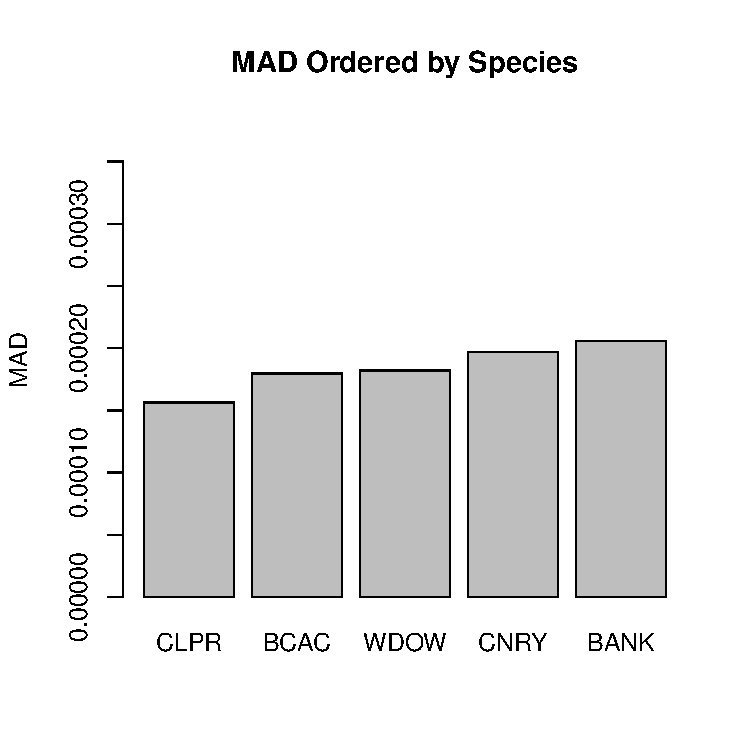
\includegraphics[width=.4\textwidth]{../sscRuns/25319781982M4U4/sppHeadMad68.pdf}
        \end{figure}
\end{frame}

%
%

%
\begin{frame}
        \begin{figure}[ht!]
        \centering
        \vspace{-0.75cm}
        \includegraphics[height=1.1\textheight]{{./postSSC/25319781982M4HC1HC3U4/margBCAC/margBCAC-0.68-Diagnostic}.pdf}
        \end{figure}   
\end{frame}

%
%

%
\begin{frame}
       \begin{figure}[ht!]
       \centering
       \vspace{-0.75cm}
       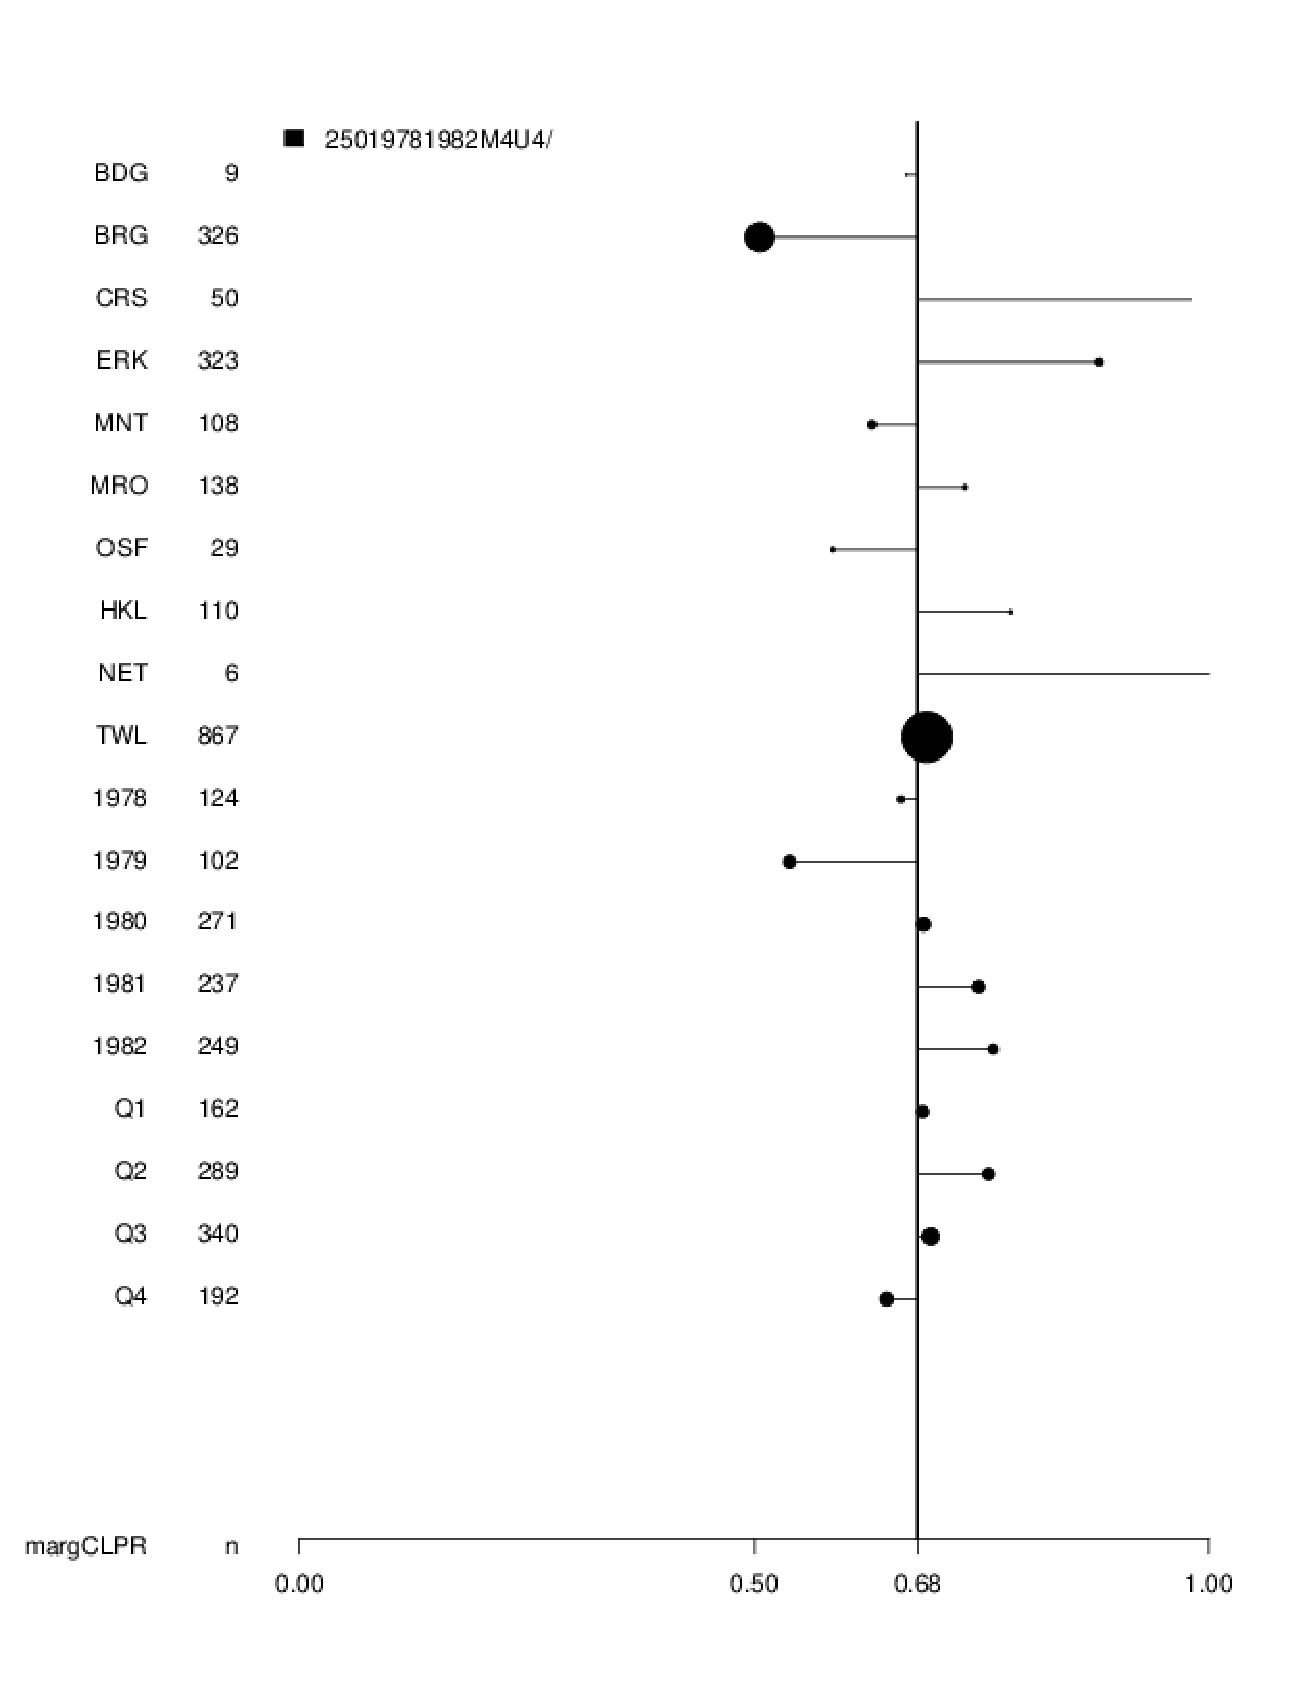
\includegraphics[height=1.1\textheight]{{./postSSC/25319781982M4HC1HC3U4/margCLPR/margCLPR-0.68-Diagnostic}.pdf}
       \end{figure}
\end{frame}

%
%

\begin{frame}{$~~~~~~~$ \href{https://github.com/gasduster99/sppComp/tree/master/sscRuns/25319781982M4HC1}{M4HC1} $~~~~~~~~~~~~~~$ \href{https://github.com/gasduster99/sppComp/tree/master/sscRuns/25319781982M4HC3}{M4HC3} $~~~~~~~~~~~~~~~~~$ \href{https://github.com/gasduster99/sppComp/tree/master/sscRuns/25319781982M4U4}{M4U4} }
        \begin{figure}[ht!]
        \centering
        \hspace*{-1cm}
        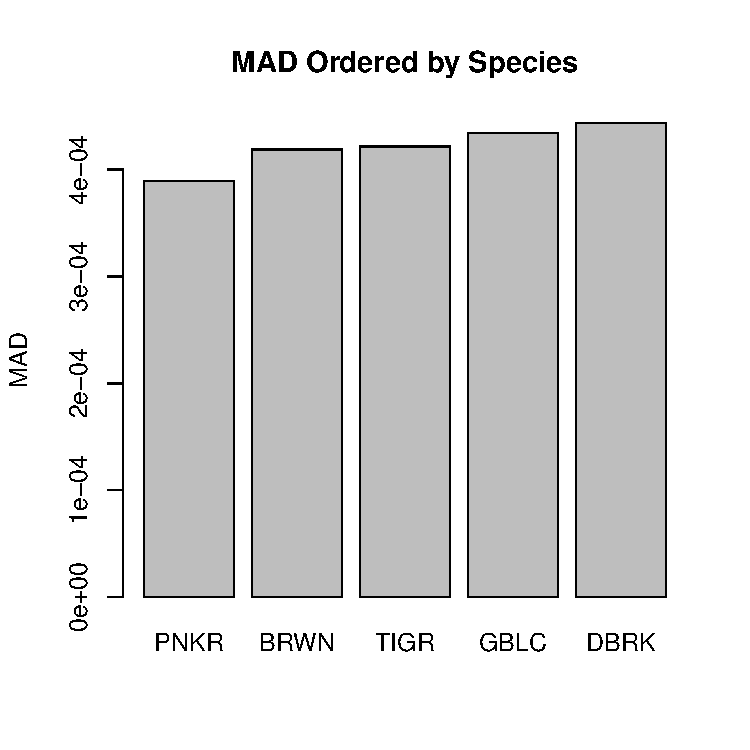
\includegraphics[width=.4\textwidth]{../sscRuns/25319781982M4HC1/sppTailMad68.pdf}
        \includegraphics[width=.4\textwidth]{../sscRuns/25319781982M4HC3/sppTailMad68.pdf}
        \includegraphics[width=.4\textwidth]{../sscRuns/25319781982M4U4/sppTailMad68.pdf}
        \end{figure}
\end{frame}

%
%

%
\begin{frame}
        \begin{figure}[ht!]
        \centering
        \vspace{-0.75cm}
        \includegraphics[height=1.1\textheight]{{./postSSC/25319781982M4HC1HC3U4/margCWCD/margCWCD-0.68-Diagnostic}.pdf}
        \end{figure}   
\end{frame}

%
%

%
\begin{frame}
       \begin{figure}[ht!]
       \centering
       \vspace{-0.75cm}
       \includegraphics[height=1.1\textheight]{{./postSSC/25319781982M4HC1HC3U4/margDBRK/margDBRK-0.68-Diagnostic}.pdf}
       \end{figure}
\end{frame}

%
%

\subsection{}
\begin{frame}{MCAT 269}
        \begin{table}[ht!]
        \centering
        \begin{tabular}[c]{@{}lcccccc@{}}
        %\toprule
        \hline
        & \href{https://github.com/gasduster99/sppComp/tree/master/sscRuns/26919781982M4}{M4} & \href{https://github.com/gasduster99/sppComp/tree/master/sscRuns/26919781982M4HC1}{M4HC1} & \href{https://github.com/gasduster99/sppComp/tree/master/sscRuns/26919781982M4HC3}{M4HC3} & \href{https://github.com/gasduster99/sppComp/tree/master/sscRuns/26919781982M4U4}{M4U4} \\ \hline
	\(\Delta\) DIC & 0.18 & 176.33 & 0.2 & 0 \\
	\(\Delta\) WAIC & 0.08 & 69.19 & 0.08 & 0 \\
	\(pr(M|y)\) & 0 & 1 & 0 & 0 \\ \hline
	\end{tabular}
        \end{table}
\end{frame}

%
%

\begin{frame}{$~~~~~~~$ \href{https://github.com/gasduster99/sppComp/tree/master/sscRuns/26919781982M4HC1}{M4HC1} $~~~~~~~~~~~~~~$ \href{https://github.com/gasduster99/sppComp/tree/master/sscRuns/26919781982M4HC3}{M4HC3} $~~~~~~~~~~~~~~~~~$ \href{https://github.com/gasduster99/sppComp/tree/master/sscRuns/26919781982M4U4}{M4U4} }
        \begin{figure}[ht!]
        \centering
        \hspace*{-1cm}
        \includegraphics[width=.4\textwidth]{../sscRuns/26919781982M4HC1/sppHeadMad68.pdf}
        \includegraphics[width=.4\textwidth]{../sscRuns/26919781982M4HC3/sppHeadMad68.pdf}
        \includegraphics[width=.4\textwidth]{../sscRuns/26919781982M4U4/sppHeadMad68.pdf}
        \end{figure}
\end{frame}

%
%

%
\begin{frame}
        \begin{figure}[ht!]
        \centering
        \vspace{-0.75cm}
        \includegraphics[height=1.1\textheight]{{./postSSC/26919781982M4HC1HC3U4/margCLPR/margCLPR-0.68-Diagnostic}.pdf}
        \end{figure}   
\end{frame}

%
%

%
\begin{frame}
       \begin{figure}[ht!]
       \centering
       \vspace{-0.75cm}
       \includegraphics[height=1.1\textheight]{{./postSSC/26919781982M4HC1HC3U4/margYTRK/margYTRK-0.68-Diagnostic}.pdf}
       \end{figure}
\end{frame}

%
%

\begin{frame}{$~~~~~~~$ \href{https://github.com/gasduster99/sppComp/tree/master/sscRuns/26919781982M4HC1}{M4HC1} $~~~~~~~~~~~~~~$ \href{https://github.com/gasduster99/sppComp/tree/master/sscRuns/26919781982M4HC3}{M4HC3} $~~~~~~~~~~~~~~~~~$ \href{https://github.com/gasduster99/sppComp/tree/master/sscRuns/26919781982M4U4}{M4U4} }
        \begin{figure}[ht!]
        \centering
        \hspace*{-1cm}
        \includegraphics[width=.4\textwidth]{../sscRuns/26919781982M4HC1/sppTailMad68.pdf}
        \includegraphics[width=.4\textwidth]{../sscRuns/26919781982M4HC3/sppTailMad68.pdf}
        \includegraphics[width=.4\textwidth]{../sscRuns/26919781982M4U4/sppTailMad68.pdf}
        \end{figure}
\end{frame}

%
%

%
\begin{frame}
        \begin{figure}[ht!]
        \centering
        \vspace{-0.75cm}
        \includegraphics[height=1.1\textheight]{{./postSSC/26919781982M4HC1HC3U4/margBCAC/margBCAC-0.68-Diagnostic}.pdf}
        \end{figure}   
\end{frame}

%
%

%
\begin{frame}
       \begin{figure}[ht!]
       \centering
       \vspace{-0.75cm}
       \includegraphics[height=1.1\textheight]{{./postSSC/26919781982M4HC1HC3U4/margWDOW/margWDOW-0.68-Diagnostic}.pdf}
       \end{figure}
\end{frame}


%
%

\section{Time Block}
\subsection{}
\begin{frame}{Time Blocks}
	$~$
\end{frame}

%
%

%
\section{Proofs}
\subsection{}
\begin{frame}{Proof: Species Comps Sum to One... as do Their Means.}
%\begin{proof}{Species Compositions Sum to One}
%
If $y_{jk}$ is the $k^{\text{th}}$ draw, $k\in\{1,...,~K\}$, of the posterior predictive weight of species $j$ in a particular stratum. Then,
%
\begin{equation}
\pi_{jk} = \frac{y_{jk}}{\sum_j y_{jk}} ~~~ \bm{y}_{k}\neq \bm{0}.
\end{equation}
The predictive mean for species $j$ is,
\begin{equation}
        \hat\pi_{j} = \frac{\sum_k^K \pi_{jk}}{K}. 
\end{equation}
Summing $\hat\pi_{j}$ across species, it follows from (1) and (2) that,
\begin{equation*}
        \hspace*{-0.8cm}
        \sum_j \hat\pi_{j} ~\substack{(2)\\=}~ \sum_j\frac{\sum_k^K \pi_{jk}}{K} = \frac{\sum_k^K \sum_j \pi_{jk}}{K}~\substack{(1)\\=}~\frac{\sum_k^K \sum_j \frac{y_{jk}}{\sum_j y_{jk}}}{K} = \frac{\sum_k^K 1}{K} = \frac{K}{K}=1. ~~~\blacksquare
\end{equation*}
%\end{proof}
%
\end{frame}

%
%

%
\subsection{}
\begin{frame}{Proof: Species Comps are Negatively Correlated.}
	%From the previous proof we have $\sum_j \pi_{j}\le 1,~\pi_j \ge 0$.\\ 
	Here we seek to show for any two species $l\neq m$, $Corr(\pi_{l}, \pi_{m})<0$.\\
	Recall:
	\begin{align*}
		Corr(\pi_{l}, \pi_{m}) &= \frac{Cov(\pi_{l}, \pi_{m})}{\sigma_{\pi_{l}}\sigma_{\pi_{m}}} ~~~ \sigma_{\pi_{l}}\ge0,~ \sigma_{\pi_{m}}\ge0 \nonumber\\
		Corr(\pi_{l}, \pi_{m}) &\le 0 \iff Cov(\pi_{l}, \pi_{m}) \le 0 \nonumber\\
		Cov(\pi_{l}, \pi_{m}) &= \mathbb{E}[(\pi_{l}-\mathbb{E}[\pi_{l}])(\pi_{m}-\mathbb{E}[\pi_{m}])] \nonumber\\ 
		&= \mathbb{E}[\pi_{l}\pi_{m}])] - \mathbb{E}[\pi_{l}]\mathbb{E}[\pi_{m}] \nonumber\\
		Cov(\pi_{l}, \pi_{m}) &\le0 \iff \mathbb{E}[\pi_{l}]\mathbb{E}[\pi_{m}] \ge \mathbb{E}[\pi_{l}\pi_{m}]
	\end{align*}
	%Consider $f(\bm{x})=\prod_i x_i : \sum_i x_i=1$. *A strictly concave function on $\sum_i x_i=1$.\\
	%Jensen's Inequality for $f$ is, $f(\mathbb{E}[\bm{x}]) \ge \mathbb{E}[f(\bm{x})]$.\\
	%Thus $\mathbb{E}[\pi_{l}]\mathbb{E}[\pi_{m}] \ge \mathbb{E}[\pi_{l}\pi_{m}]$ with equality only when $\pi$ is a constant. 
\end{frame}

%
%

%
\begin{frame}{Proof: Species Comps are Negatively Correlated Cont.}
	\mbox{Consider the strictly concave function: $f(\bm{x})=\prod_i x_i : \sum_i x_i \le 1,~x_i \ge 0$.}\\  	
	Jensen's Inequality for $f$ is,
	\begin{equation}
		f(\mathbb{E}[\bm{x}]) \ge \mathbb{E}[f(\bm{x})].
		\label{jensen}
	\end{equation}
	\mbox{From the previous proof: $\sum_j \pi_{j}\le 1,~\pi_j \ge 0$ and $\sum_j \hat\pi_{j}\le 1,~\hat\pi_j \ge 0$.}\\
        Thus applying (\ref{jensen}) to $\bm{\pi}$ gives  
	\begin{equation}
		\mathbb{E}[\pi_{l}]\mathbb{E}[\pi_{m}] \ge \mathbb{E}[\pi_{l}\pi_{m}]
	\end{equation}
	with equality only if $\pi$ is a constant. Since $\pi$ is never a constant, 
	\begin{align*}
		\mathbb{E}[\pi_{l}]\mathbb{E}[\pi_{m}] &> \mathbb{E}[\pi_{l}\pi_{m}]\\
		Cov(\pi_{l}, \pi_{m})&<0\\ 
		Corr(\pi_{l}, \pi_{m})&<0. ~~~\blacksquare
	\end{align*} 
\end{frame}

%
\end{document}
